\documentclass{jlreq}

\usepackage{titlesec}
\usepackage{listings}
\usepackage{fancyhdr}

% url
\usepackage{url}

% \adjustbox
\usepackage{adjustbox}

% tcolorboxの設定
\usepackage[most]{tcolorbox} 
\tcbuselibrary{breakable}
\tcbuselibrary{skins}
\tcbuselibrary{listingsutf8}
% タイトルのフォーマットを変更
\titleformat{\title}
  {\centering\Huge\bfseries}
  {}
  {0em} 
  {}

\titleformat{\subtitle}
  {\centering\Large\itshape}
  {}
  {0em}
  {}

\titleformat{\subsubsection}[block]
  {\normalfont\normalsize\bfseries}
  {\arabic{subsubsection}.}
  {1em}
  {}

\titleformat{\section}[block]
  {\normalfont\large\bfseries}
  {\Roman{section}.}
  {1em} 
  {}
  [\titleline{\titlerule[1pt]}]

\titleformat{\subsection}[block]
  {\normalfont\normalsize\bfseries}
  {\roman{subsection}.}
  {1em}
  {}

% listingsの設定

\renewcommand{\lstlistingname}{コード}

\lstset{
	breaklines = true,
	language = Python,
	keywordstyle = {\bfseries \color[cmyk]{0,1,0,0}},
	commentstyle = {\itshape \color[cmyk]{1,0.4,1,0}},
	numbers = left,
	numberstyle = \tiny,
	stepnumber = 1,
	% frameとnumberの間の距離
	numbersep = 10pt,
	frame = single,
	basicstyle = \ttfamily,
	tabsize = 2,
	captionpos = t,
	backgroundcolor={\color[gray]{.90}},
	showstringspaces = false,
}

% headerの設定
\pagestyle{fancy}
\fancyhf{}

\fancyhead[RO,RE]{\rightmark}
\fancyhead[LO,LE]{\leftmark} 
\fancyfoot[C]{\thepage}

% tikzの設定
\usepackage{tikz}

% 定理環境
\newtcolorbox{theorembox}[1][]{
    enhanced,
    colback=white!95!green,
    colframe=green!40!black,
    coltitle=black,
    fonttitle=\bfseries,
    title=#1,
    attach boxed title to top left={yshift=-2mm, xshift=2mm},
    boxed title style={colback=green!30!white, size=small},
    drop fuzzy shadow,
    boxrule=0.5mm,
    sharp corners,
    top=4mm, bottom=4mm,
}

\newtcolorbox{definitionbox}[1][]{
    enhanced,
    title=#1, 
    attach boxed title to top left, 
    colback=white!95!blue,
    colbacktitle=white!10!blue!50!black,
    drop fuzzy shadow,
    boxrule=0.25mm,
}
% 問題用のボックス環境
\newtcolorbox{problem}[1][]{enhanced,
  colback=white!85!gray,
  drop fuzzy shadow,
  boxrule=0.3mm,
  arc=0mm,
  left=0pt,
  top=0pt,
  sharp corners,
  width=\textwidth,
  title=\textbf{問題},
  #1
}

\begin{document}
\section{グラフの用語整理}
グラフはノードとエッジからなるデータ構造です。グラフの用語を整理します。

\subsection{ツリー(木)}
ツリーは閉路を持たない連結なグラフです。ツリーは以下の性質を持ちます。
\begin{itemize}
  \item 連結なグラフである
  \item 閉路を持たない
\end{itemize}

ノードの数が$n$であるグラフ$G$が木であることは、以下の条件とも同値です。

\begin{itemize}
  \item $G$には閉路がなく、$n-1$本のエッジを持つ
  \item $G$は連結であり、$n-1$本のエッジを持つ
  \item $G$の任意の2点を結ぶ経路はただ1つ存在する
\end{itemize}

\subsection{無向グラフと有向グラフ}
無向グラフはエッジに向きがないグラフです。有向グラフはエッジに向きがあるグラフです。
\vspace{0.5cm}

\begin{center}
  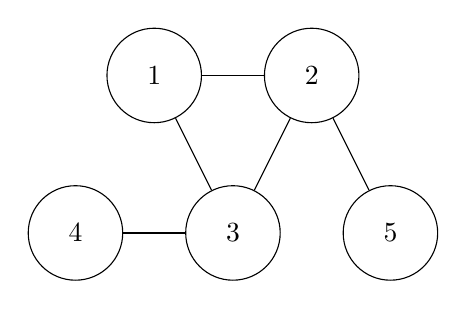
\begin{tikzpicture}[scale=1]
    % ノードの定義
    \node[circle, draw, minimum size=1.2cm] (A) at (0, 0) {1}; 
    \node[circle, draw, minimum size=1.2cm] (B) at (2, 0) {2};
    \node[circle, draw, minimum size=1.2cm] (C) at (1, -2) {3};
    \node[circle, draw, minimum size=1.2cm] (D) at (-1, -2) {4};
    \node[circle, draw, minimum size=1.2cm] (E) at (3, -2) {5};

    % 無向エッジを引く
    \draw (A) -- (B);
    \draw (A) -- (C);
    \draw (B) -- (C);
    \draw (C) -- (D);
    \draw (B) -- (E);

  \end{tikzpicture}
\end{center}
\begin{center}
  無向グラフ
\end{center}
\vspace{0.5cm}

\begin{center}
  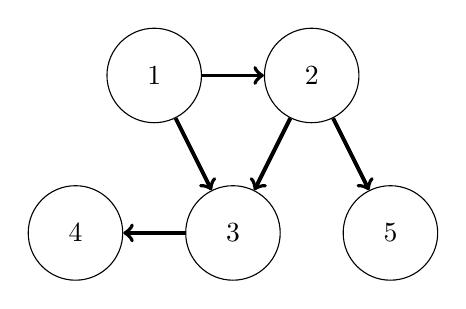
\begin{tikzpicture}[scale=1]
    % ノードの定義
    \node[circle, draw, minimum size=1.2cm] (A) at (0, 0) {1}; 
    \node[circle, draw, minimum size=1.2cm] (B) at (2, 0) {2};
    \node[circle, draw, minimum size=1.2cm] (C) at (1, -2) {3};
    \node[circle, draw, minimum size=1.2cm] (D) at (-1, -2) {4};
    \node[circle, draw, minimum size=1.2cm] (E) at (3, -2) {5};

    % 太い有向エッジを引く
    \draw[->, line width=0.5mm] (A) -- (B);
    \draw[->, line width=0.5mm] (A) -- (C);
    \draw[->, line width=0.5mm] (B) -- (C);
    \draw[->, line width=0.5mm] (C) -- (D);
    \draw[->, line width=0.5mm] (B) -- (E);

  \end{tikzpicture}
\end{center}

\begin{center}
  有向グラフ
\end{center}

\subsection{重み付きグラフ}
重み付きグラフはエッジに重みがついたグラフです。重みはエッジのコストや距離を表します。

\begin{center}
  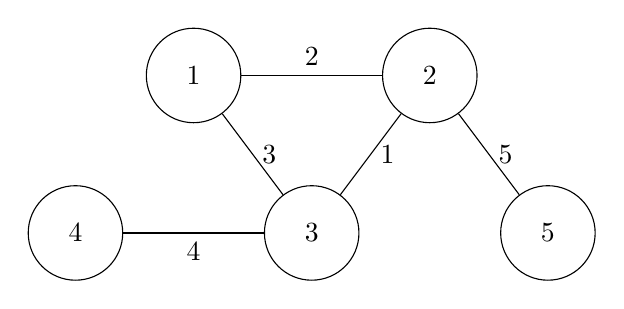
\begin{tikzpicture}[scale=1, auto, node distance=2cm, every loop/.style={}]
    % ノードの定義
    \node[circle, draw, minimum size=1.2cm] (A) at (0, 0) {1}; 
    \node[circle, draw, minimum size=1.2cm] (B) at (3, 0) {2};
    \node[circle, draw, minimum size=1.2cm] (C) at (1.5, -2) {3};
    \node[circle, draw, minimum size=1.2cm] (D) at (-1.5, -2) {4};
    \node[circle, draw, minimum size=1.2cm] (E) at (4.5, -2) {5};

    % エッジと重みを描く
    \draw[-] (A) -- (B) node[midway, above] {2};
    \draw[-] (A) -- (C) node[midway, right] {3};
    \draw[-] (B) -- (C) node[midway, right] {1};
    \draw[-] (C) -- (D) node[midway, below] {4};
    \draw[-] (B) -- (E) node[midway, right] {5};

  \end{tikzpicture}
\end{center}

\subsection{隣接行列と隣接リスト}

隣接行列と隣接リストはグラフを表現するためのデータ構造です。
以下のグラフを例にして、隣接行列と隣接リストを示します。

\begin{center}
  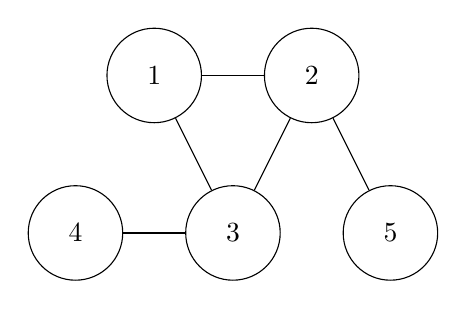
\begin{tikzpicture}[scale=1]
    % ノードの定義
    \node[circle, draw, minimum size=1.2cm] (A) at (0, 0) {1}; 
    \node[circle, draw, minimum size=1.2cm] (B) at (2, 0) {2};
    \node[circle, draw, minimum size=1.2cm] (C) at (1, -2) {3};
    \node[circle, draw, minimum size=1.2cm] (D) at (-1, -2) {4};
    \node[circle, draw, minimum size=1.2cm] (E) at (3, -2) {5};

    % 無向エッジを引く
    \draw (A) -- (B);
    \draw (A) -- (C);
    \draw (B) -- (C);
    \draw (C) -- (D);
    \draw (B) -- (E);

  \end{tikzpicture}
\end{center}
\subsubsection*{隣接行列}

隣接行列はグラフのエッジを行列で表現したものです。$(i, j)$成分が1のとき、ノード$i$とノード$j$がエッジで結ばれていることを表します。下の図では
隣接行列は1-indexedで表現しています。

\[
\begin{pmatrix}
0 & 1 & 1 & 0 & 0 \\
1 & 0 & 1 & 0 & 1 \\
1 & 1 & 0 & 1 & 0 \\
0 & 0 & 1 & 0 & 0 \\
0 & 1 & 0 & 0 & 0 \\
\end{pmatrix}
\]

\subsubsection*{隣接リスト}
隣接リストは各ノードに隣接するノードをリストで表現したものです。

\begin{itemize}
  \item 1: 2, 3
  \item 2: 1, 3, 5
  \item 3: 1, 2, 4
  \item 4: 3
  \item 5: 2
\end{itemize}

\newpage

グラフの基本として、深さ優先探索(DFS)と幅優先探索(BFS)というグラフの探索アルゴリズムを扱います。
\section{幅優先探索(BFS)}
BFSは、後戻りしないように、可能性のあるルートすべてにおいて1ステップずつ行くアルゴリズムです。BFS
の例を見てみましょう。

\vspace{0.5cm}

\begin{center}
  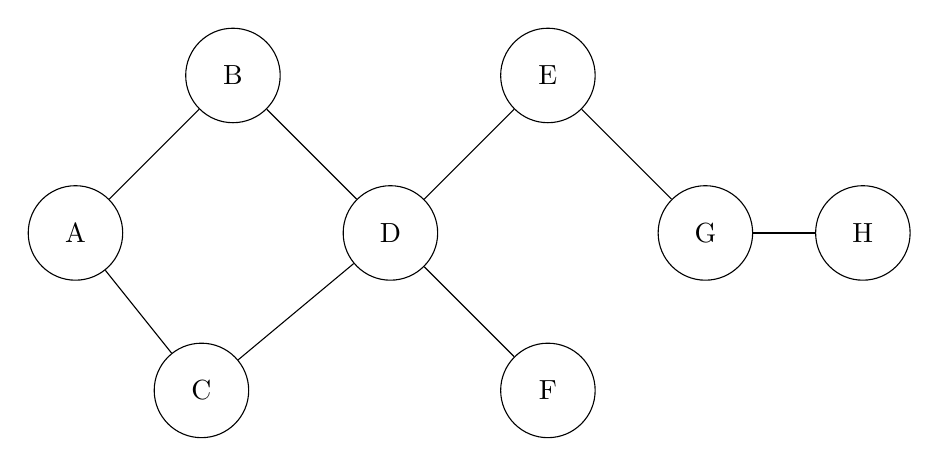
\begin{tikzpicture}
    % ノード
    \node[circle, draw, minimum size=1.2cm] (A) at (-4, 0) {A};
    \node[circle, draw, minimum size=1.2cm] (B) at (-2, 2) {B};
    \node[circle, draw, minimum size=1.2cm] (C) at (-2.4, -2) {C};
    \node[circle, draw, minimum size=1.2cm] (D) at (0, 0) {D};
    \node[circle, draw, minimum size=1.2cm] (E) at (2, 2) {E};
    \node[circle, draw, minimum size=1.2cm] (F) at (2, -2) {F};
    \node[circle, draw, minimum size=1.2cm] (G) at (4, 0) {G};
    \node[circle, draw, minimum size=1.2cm] (H) at (6, 0) {H};

    % エッジ
    \draw (A) -- (B);
    \draw (A) -- (C);
    \draw (C) -- (D);
    \draw (B) -- (D);
    \draw (D) -- (E);
    \draw (D) -- (F);
    \draw (E) -- (G);
    \draw (G) -- (H);
  \end{tikzpicture}
\end{center}
\vspace{0.5cm}

Aからスタートします。

\vspace{0.5cm}

\begin{center}
  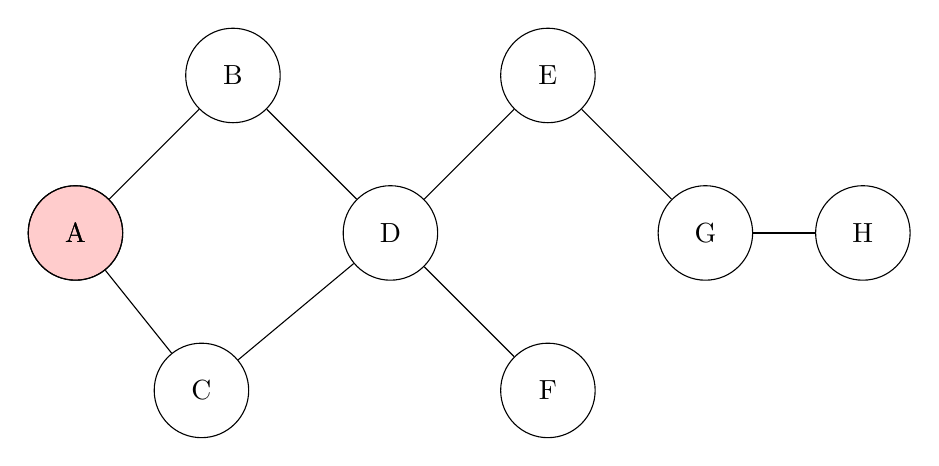
\begin{tikzpicture}
    % 探索済みノードに赤色を塗る
    \node[circle, draw, minimum size=1.2cm, fill=red!20] (A) at (-4, 0) {A};

    % ノード
    \node[circle, draw, minimum size=1.2cm] (A) at (-4, 0) {A};
    \node[circle, draw, minimum size=1.2cm] (B) at (-2, 2) {B};
    \node[circle, draw, minimum size=1.2cm] (C) at (-2.4, -2) {C};
    \node[circle, draw, minimum size=1.2cm] (D) at (0, 0) {D};
    \node[circle, draw, minimum size=1.2cm] (E) at (2, 2) {E};
    \node[circle, draw, minimum size=1.2cm] (F) at (2, -2) {F};
    \node[circle, draw, minimum size=1.2cm] (G) at (4, 0) {G};
    \node[circle, draw, minimum size=1.2cm] (H) at (6, 0) {H};

    % エッジ
    \draw (A) -- (B);
    \draw (A) -- (C);
    \draw (C) -- (D);
    \draw (B) -- (D);
    \draw (D) -- (E);
    \draw (D) -- (F);
    \draw (E) -- (G);
    \draw (G) -- (H);
  \end{tikzpicture}
\end{center}

次にAと繋がっているノードBとCを探索します。

\vspace{0.5cm}

\begin{center}
  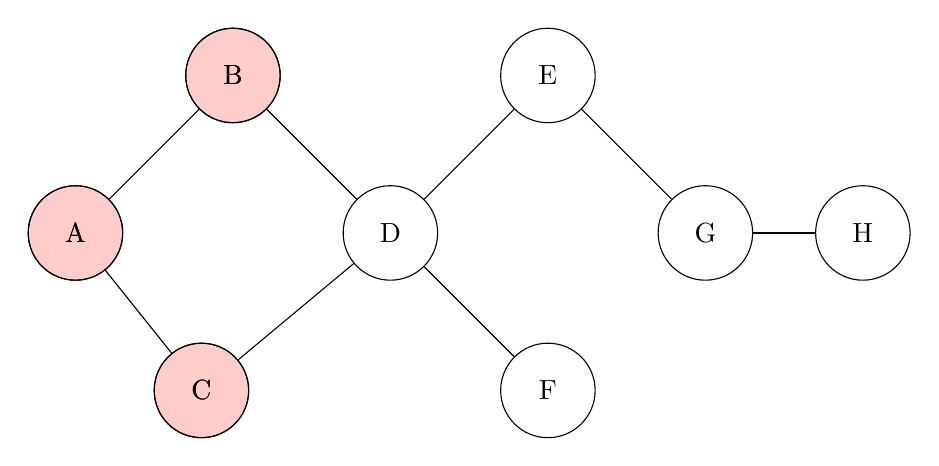
\begin{tikzpicture}
    % 探索済みノードに赤色を塗る
    \node[circle, draw, minimum size=1.2cm, fill=red!20] (A) at (-4, 0) {A};
    \node[circle, draw, minimum size=1.2cm, fill=red!20] (B) at (-2, 2) {B};
    \node[circle, draw, minimum size=1.2cm, fill=red!20] (C) at (-2.4, -2) {C};

    % ノード
    \node[circle, draw, minimum size=1.2cm] (A) at (-4, 0) {A};
    \node[circle, draw, minimum size=1.2cm] (B) at (-2, 2) {B};
    \node[circle, draw, minimum size=1.2cm] (C) at (-2.4, -2) {C};
    \node[circle, draw, minimum size=1.2cm] (D) at (0, 0) {D};
    \node[circle, draw, minimum size=1.2cm] (E) at (2, 2) {E};
    \node[circle, draw, minimum size=1.2cm] (F) at (2, -2) {F};
    \node[circle, draw, minimum size=1.2cm] (G) at (4, 0) {G};
    \node[circle, draw, minimum size=1.2cm] (H) at (6, 0) {H};

    % エッジ
    \draw (A) -- (B);
    \draw (A) -- (C);
    \draw (C) -- (D);
    \draw (B) -- (D);
    \draw (D) -- (E);
    \draw (D) -- (F);
    \draw (E) -- (G);
    \draw (G) -- (H);
  \end{tikzpicture}
\end{center}
\vspace{0.5cm}

Aの探索が終わったので、次にBとCの探索を行います。今回はBから探索します。BとCは同じ深さにあるので、
どちらから探索しても問題ありません。BにはDが繋がっているので、Dを探索します。Cから
探索を始めようとすると、すでにDはすでに探索済みなので、探索を行いません。

\begin{center}
  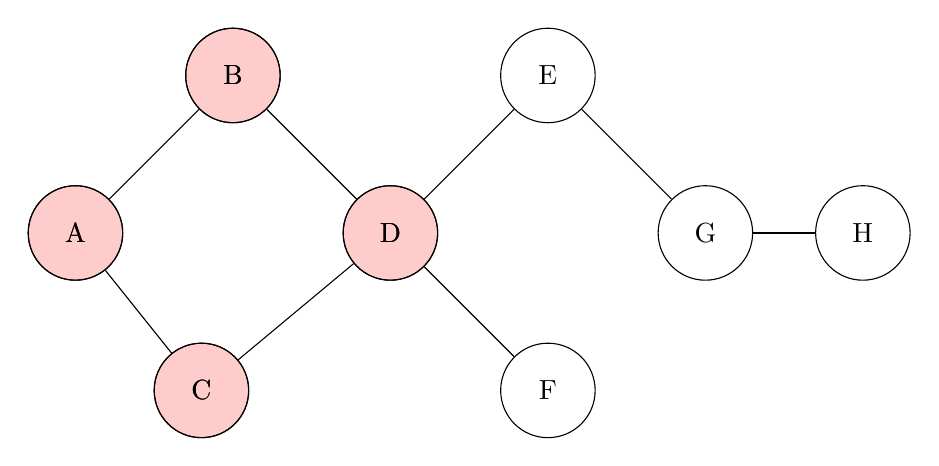
\begin{tikzpicture}
    % 探索済みノードに赤色を塗る
    \node[circle, draw, minimum size=1.2cm, fill=red!20] (A) at (-4, 0) {A};
    \node[circle, draw, minimum size=1.2cm, fill=red!20] (B) at (-2, 2) {B};
    \node[circle, draw, minimum size=1.2cm, fill=red!20] (C) at (-2.4, -2) {C};
    \node[circle, draw, minimum size=1.2cm, fill=red!20] (D) at (0, 0) {D};

    % ノード
    \node[circle, draw, minimum size=1.2cm] (A) at (-4, 0) {A};
    \node[circle, draw, minimum size=1.2cm] (B) at (-2, 2) {B};
    \node[circle, draw, minimum size=1.2cm] (C) at (-2.4, -2) {C};
    \node[circle, draw, minimum size=1.2cm] (D) at (0, 0) {D};
    \node[circle, draw, minimum size=1.2cm] (E) at (2, 2) {E};
    \node[circle, draw, minimum size=1.2cm] (F) at (2, -2) {F};
    \node[circle, draw, minimum size=1.2cm] (G) at (4, 0) {G};
    \node[circle, draw, minimum size=1.2cm] (H) at (6, 0) {H};

    % エッジ
    \draw (A) -- (B);
    \draw (A) -- (C);
    \draw (C) -- (D);
    \draw (B) -- (D);
    \draw (D) -- (E);
    \draw (D) -- (F);
    \draw (E) -- (G);
    \draw (G) -- (H);
  \end{tikzpicture}
\end{center}
\vspace{0.5cm}

次にDから探索を行います。DにはEとFが繋がっているので、EとFを探索します。

\vspace{0.5cm}
\begin{center}
  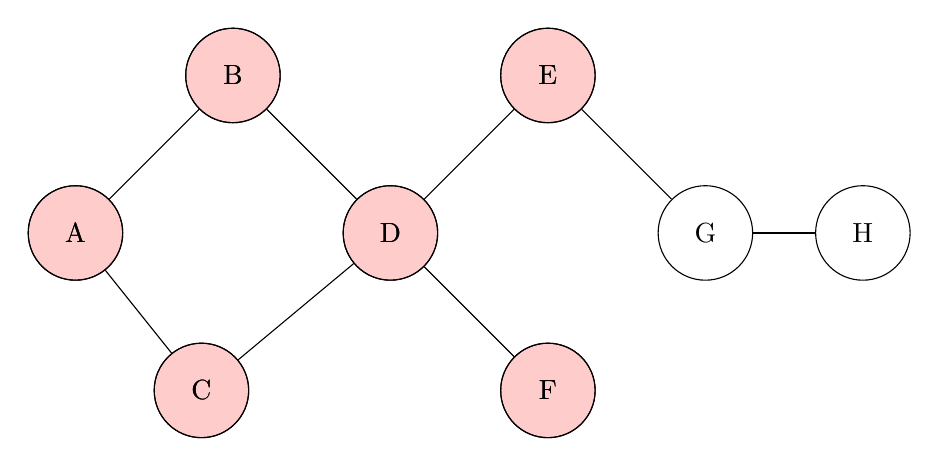
\begin{tikzpicture}
    % 探索済みノードに赤色を塗る
    \node[circle, draw, minimum size=1.2cm, fill=red!20] (A) at (-4, 0) {A};
    \node[circle, draw, minimum size=1.2cm, fill=red!20] (B) at (-2, 2) {B};
    \node[circle, draw, minimum size=1.2cm, fill=red!20] (C) at (-2.4, -2) {C};
    \node[circle, draw, minimum size=1.2cm, fill=red!20] (D) at (0, 0) {D};
    \node[circle, draw, minimum size=1.2cm, fill=red!20] (E) at (2, 2) {E};
    \node[circle, draw, minimum size=1.2cm, fill=red!20] (F) at (2, -2) {F};

    % ノード
    \node[circle, draw, minimum size=1.2cm] (A) at (-4, 0) {A};
    \node[circle, draw, minimum size=1.2cm] (B) at (-2, 2) {B};
    \node[circle, draw, minimum size=1.2cm] (C) at (-2.4, -2) {C};
    \node[circle, draw, minimum size=1.2cm] (D) at (0, 0) {D};
    \node[circle, draw, minimum size=1.2cm] (E) at (2, 2) {E};
    \node[circle, draw, minimum size=1.2cm] (F) at (2, -2) {F};
    \node[circle, draw, minimum size=1.2cm] (G) at (4, 0) {G};
    \node[circle, draw, minimum size=1.2cm] (H) at (6, 0) {H};

    % エッジ
    \draw (A) -- (B);
    \draw (A) -- (C);
    \draw (C) -- (D);
    \draw (B) -- (D);
    \draw (D) -- (E);
    \draw (D) -- (F);
    \draw (E) -- (G);
    \draw (G) -- (H);
  \end{tikzpicture}
\end{center}
\vspace{0.5cm}

最後にGとHを探索します。

\begin{center}
  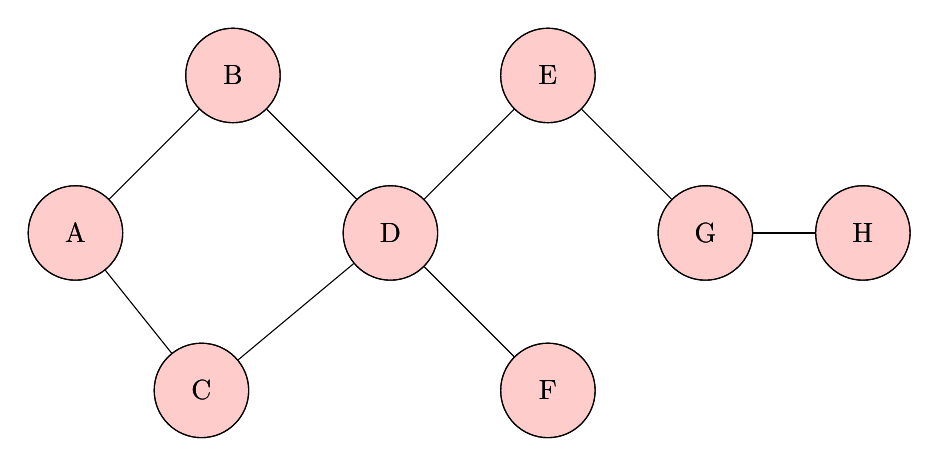
\begin{tikzpicture}
    % 探索済みノードに赤色を塗る
    \node[circle, draw, minimum size=1.2cm, fill=red!20] (A) at (-4, 0) {A};
    \node[circle, draw, minimum size=1.2cm, fill=red!20] (B) at (-2, 2) {B};
    \node[circle, draw, minimum size=1.2cm, fill=red!20] (C) at (-2.4, -2) {C};
    \node[circle, draw, minimum size=1.2cm, fill=red!20] (D) at (0, 0) {D};
    \node[circle, draw, minimum size=1.2cm, fill=red!20] (E) at (2, 2) {E};
    \node[circle, draw, minimum size=1.2cm, fill=red!20] (F) at (2, -2) {F};
    \node[circle, draw, minimum size=1.2cm, fill=red!20] (G) at (4, 0) {G};
    \node[circle, draw, minimum size=1.2cm, fill=red!20] (H) at (6, 0) {H};

    % ノード
    \node[circle, draw, minimum size=1.2cm] (A) at (-4, 0) {A};
    \node[circle, draw, minimum size=1.2cm] (B) at (-2, 2) {B};
    \node[circle, draw, minimum size=1.2cm] (C) at (-2.4, -2) {C};
    \node[circle, draw, minimum size=1.2cm] (D) at (0, 0) {D};
    \node[circle, draw, minimum size=1.2cm] (E) at (2, 2) {E};
    \node[circle, draw, minimum size=1.2cm] (F) at (2, -2) {F};
    \node[circle, draw, minimum size=1.2cm] (G) at (4, 0) {G};
    \node[circle, draw, minimum size=1.2cm] (H) at (6, 0) {H};

    % エッジ
    \draw (A) -- (B);
    \draw (A) -- (C);
    \draw (C) -- (D);
    \draw (B) -- (D);
    \draw (D) -- (E);
    \draw (D) -- (F);
    \draw (E) -- (G);
    \draw (G) -- (H);
  \end{tikzpicture}
\end{center}
\vspace{0.5cm}

これでグラフの探索が終了しました。BFSはスタート地点からの最短距離を求めることができます。

\subsection{BFSの実装}
BFSの実装はキューを用いて行います。実装のポイントは以下の通りです。

\begin{itemize}
  \item キューを用いて、次に探索するノードを管理する
  \item 探索済みのノードを管理するために、配列を用いる
\end{itemize}

隣接リストでも隣接行列でも実装できますが、隣接リストの方が実装が簡単です。また0-indexedで実装している
ことに注意してください。

\begin{lstlisting}[caption=深さ優先探索ヒープの実装, label=bfs, frame=TRBL, label={bfs}]
from collections import deque

  def bfs(graph: list[list[int]], start: int) -> list[bool]:
      visited = [False] * len(graph)
      todo = deque()
      
      # スタート地点で初期化
      todo.append(start)
      
      while todo:
          node = todo.popleft()
          visited[node] = True
          
          for next_node in graph[node]:
              if not visited[next_node]:
                  todo.append(next_node)
                  
      return visited
\end{lstlisting}

\newpage

\section{深さ優先探索(DFS)}
DFSは、スタート地点から次のノードに進み、進んだノードに繋がっているノードを行けなくなるまで探索するアルゴリズムです。
先ほどのグラフを例にして、DFSの探索を行います。

最初はAから探索を行います。

\vspace{0.5cm}

\begin{center}
  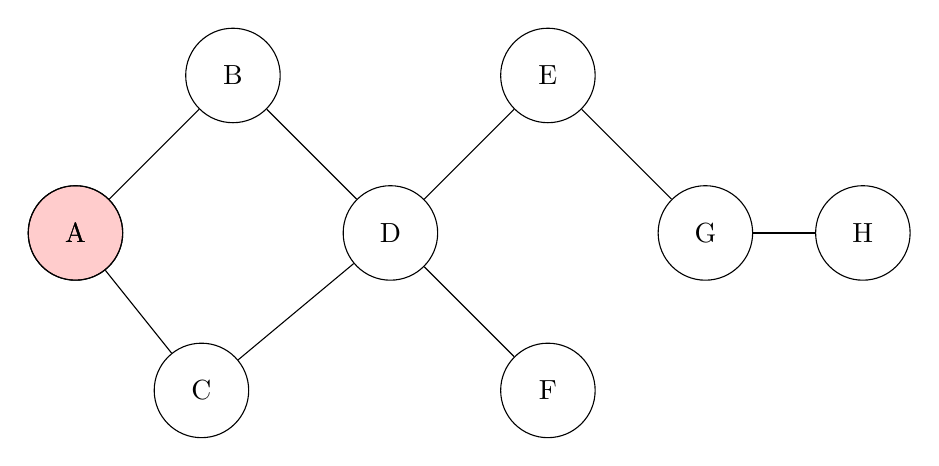
\begin{tikzpicture}
    % 探索済みノードに赤色を塗る
    \node[circle, draw, minimum size=1.2cm, fill=red!20] (A) at (-4, 0) {A};
    % ノード
    \node[circle, draw, minimum size=1.2cm] (A) at (-4, 0) {A};
    \node[circle, draw, minimum size=1.2cm] (B) at (-2, 2) {B};
    \node[circle, draw, minimum size=1.2cm] (C) at (-2.4, -2) {C};
    \node[circle, draw, minimum size=1.2cm] (D) at (0, 0) {D};
    \node[circle, draw, minimum size=1.2cm] (E) at (2, 2) {E};
    \node[circle, draw, minimum size=1.2cm] (F) at (2, -2) {F};
    \node[circle, draw, minimum size=1.2cm] (G) at (4, 0) {G};
    \node[circle, draw, minimum size=1.2cm] (H) at (6, 0) {H};

    % エッジ
    \draw (A) -- (B);
    \draw (A) -- (C);
    \draw (C) -- (D);
    \draw (B) -- (D);
    \draw (D) -- (E);
    \draw (D) -- (F);
    \draw (E) -- (G);
    \draw (G) -- (H);
  \end{tikzpicture}
\end{center}

次にAと繋がっているノードBを探索します。

\vspace{0.5cm}

\begin{center}
  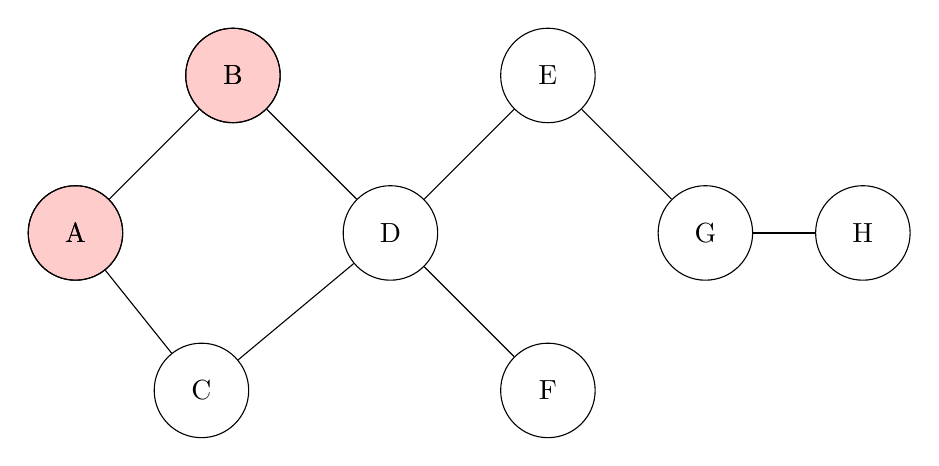
\begin{tikzpicture}
    % 探索済みノードに赤色を塗る
    \node[circle, draw, minimum size=1.2cm, fill=red!20] (A) at (-4, 0) {A};
    \node[circle, draw, minimum size=1.2cm, fill=red!20] (B) at (-2, 2) {B};
    % ノード
    \node[circle, draw, minimum size=1.2cm] (A) at (-4, 0) {A};
    \node[circle, draw, minimum size=1.2cm] (B) at (-2, 2) {B};
    \node[circle, draw, minimum size=1.2cm] (C) at (-2.4, -2) {C};
    \node[circle, draw, minimum size=1.2cm] (D) at (0, 0) {D};
    \node[circle, draw, minimum size=1.2cm] (E) at (2, 2) {E};
    \node[circle, draw, minimum size=1.2cm] (F) at (2, -2) {F};
    \node[circle, draw, minimum size=1.2cm] (G) at (4, 0) {G};
    \node[circle, draw, minimum size=1.2cm] (H) at (6, 0) {H};

    % エッジ
    \draw (A) -- (B);
    \draw (A) -- (C);
    \draw (C) -- (D);
    \draw (B) -- (D);
    \draw (D) -- (E);
    \draw (D) -- (F);
    \draw (E) -- (G);
    \draw (G) -- (H);
  \end{tikzpicture}
\end{center}

\vspace{0.5cm}

BFSではCを次に探索しますが、DFSではBに繋がっているDを探索します。

\vspace{0.5cm}

\begin{center}
  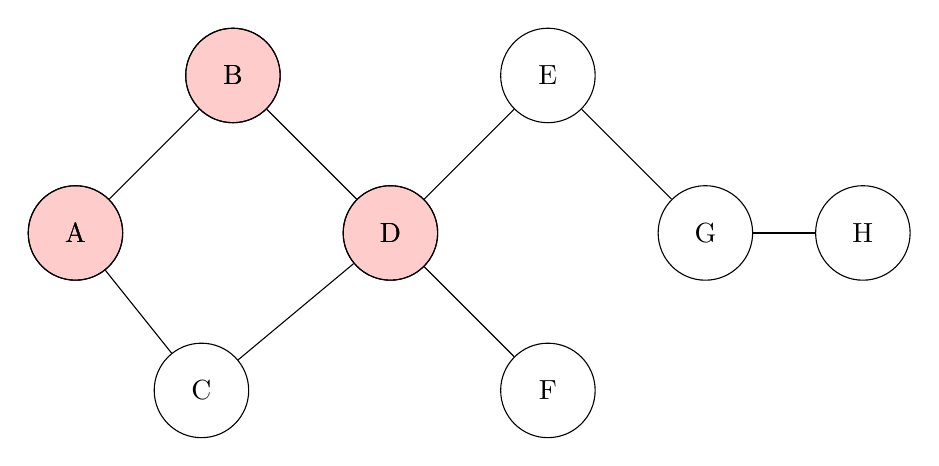
\begin{tikzpicture}
    % 探索済みノードに赤色を塗る
    \node[circle, draw, minimum size=1.2cm, fill=red!20] (A) at (-4, 0) {A};
    \node[circle, draw, minimum size=1.2cm, fill=red!20] (B) at (-2, 2) {B};
    \node[circle, draw, minimum size=1.2cm, fill=red!20] (D) at (0, 0) {D};
    % ノード
    \node[circle, draw, minimum size=1.2cm] (A) at (-4, 0) {A};
    \node[circle, draw, minimum size=1.2cm] (B) at (-2, 2) {B};
    \node[circle, draw, minimum size=1.2cm] (C) at (-2.4, -2) {C};
    \node[circle, draw, minimum size=1.2cm] (D) at (0, 0) {D};
    \node[circle, draw, minimum size=1.2cm] (E) at (2, 2) {E};
    \node[circle, draw, minimum size=1.2cm] (F) at (2, -2) {F};
    \node[circle, draw, minimum size=1.2cm] (G) at (4, 0) {G};
    \node[circle, draw, minimum size=1.2cm] (H) at (6, 0) {H};

    % エッジ
    \draw (A) -- (B);
    \draw (A) -- (C);
    \draw (C) -- (D);
    \draw (B) -- (D);
    \draw (D) -- (E);
    \draw (D) -- (F);
    \draw (E) -- (G);
    \draw (G) -- (H);
  \end{tikzpicture}
\end{center}

\vspace{0.5cm}

次にDに繋がっているEを探索します。

\begin{center}
  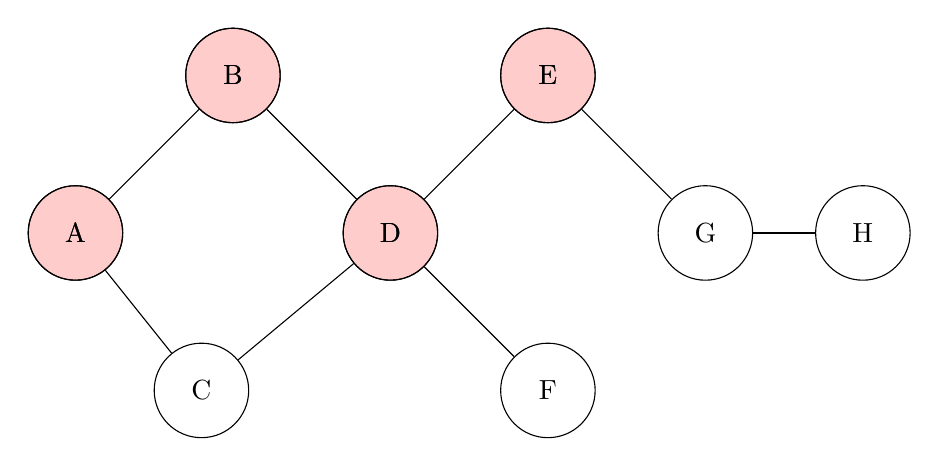
\begin{tikzpicture}
    % 探索済みノードに赤色を塗る
    \node[circle, draw, minimum size=1.2cm, fill=red!20] (A) at (-4, 0) {A};
    \node[circle, draw, minimum size=1.2cm, fill=red!20] (B) at (-2, 2) {B};
    \node[circle, draw, minimum size=1.2cm, fill=red!20] (D) at (0, 0) {D};
    \node[circle, draw, minimum size=1.2cm, fill=red!20] (E) at (2, 2) {E};
    % ノード
    \node[circle, draw, minimum size=1.2cm] (A) at (-4, 0) {A};
    \node[circle, draw, minimum size=1.2cm] (B) at (-2, 2) {B};
    \node[circle, draw, minimum size=1.2cm] (C) at (-2.4, -2) {C};
    \node[circle, draw, minimum size=1.2cm] (D) at (0, 0) {D};
    \node[circle, draw, minimum size=1.2cm] (E) at (2, 2) {E};
    \node[circle, draw, minimum size=1.2cm] (F) at (2, -2) {F};
    \node[circle, draw, minimum size=1.2cm] (G) at (4, 0) {G};
    \node[circle, draw, minimum size=1.2cm] (H) at (6, 0) {H};

    % エッジ
    \draw (A) -- (B);
    \draw (A) -- (C);
    \draw (C) -- (D);
    \draw (B) -- (D);
    \draw (D) -- (E);
    \draw (D) -- (F);
    \draw (E) -- (G);
    \draw (G) -- (H);
  \end{tikzpicture}
\end{center}

これ以上ノードがないノードHまで探索していきます。

\begin{center}
  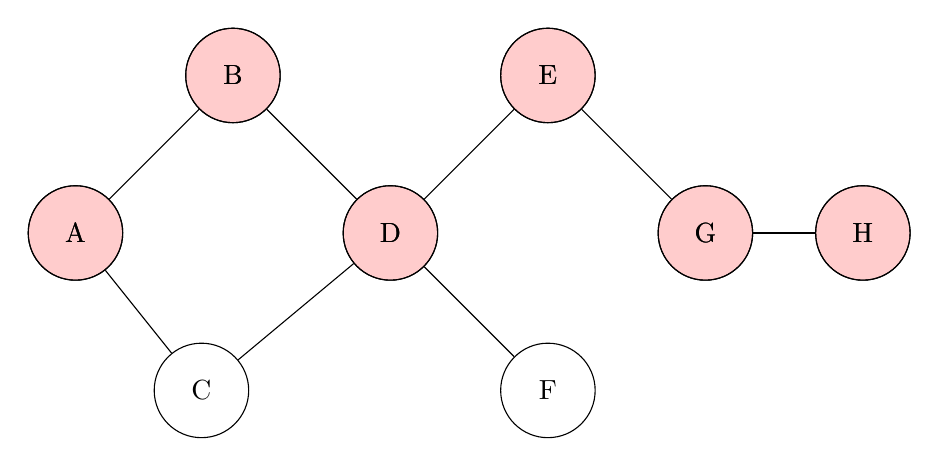
\begin{tikzpicture}
    % 探索済みノードに赤色を塗る
    \node[circle, draw, minimum size=1.2cm, fill=red!20] (A) at (-4, 0) {A};
    \node[circle, draw, minimum size=1.2cm, fill=red!20] (B) at (-2, 2) {B};
    \node[circle, draw, minimum size=1.2cm, fill=red!20] (D) at (0, 0) {D};
    \node[circle, draw, minimum size=1.2cm, fill=red!20] (E) at (2, 2) {E};
    \node[circle, draw, minimum size=1.2cm, fill=red!20] (G) at (4, 0) {G};
    \node[circle, draw, minimum size=1.2cm, fill=red!20] (H) at (6, 0) {H};
    % ノード
    \node[circle, draw, minimum size=1.2cm] (A) at (-4, 0) {A};
    \node[circle, draw, minimum size=1.2cm] (B) at (-2, 2) {B};
    \node[circle, draw, minimum size=1.2cm] (C) at (-2.4, -2) {C};
    \node[circle, draw, minimum size=1.2cm] (D) at (0, 0) {D};
    \node[circle, draw, minimum size=1.2cm] (E) at (2, 2) {E};
    \node[circle, draw, minimum size=1.2cm] (F) at (2, -2) {F};
    \node[circle, draw, minimum size=1.2cm] (G) at (4, 0) {G};
    \node[circle, draw, minimum size=1.2cm] (H) at (6, 0) {H};

    % エッジ
    \draw (A) -- (B);
    \draw (A) -- (C);
    \draw (C) -- (D);
    \draw (B) -- (D);
    \draw (D) -- (E);
    \draw (D) -- (F);
    \draw (E) -- (G);
    \draw (G) -- (H);
  \end{tikzpicture}
\end{center}

\vspace{0.5cm}
移動する余地の残っているFを探索します。

\vspace{0.5cm}

\begin{center}
  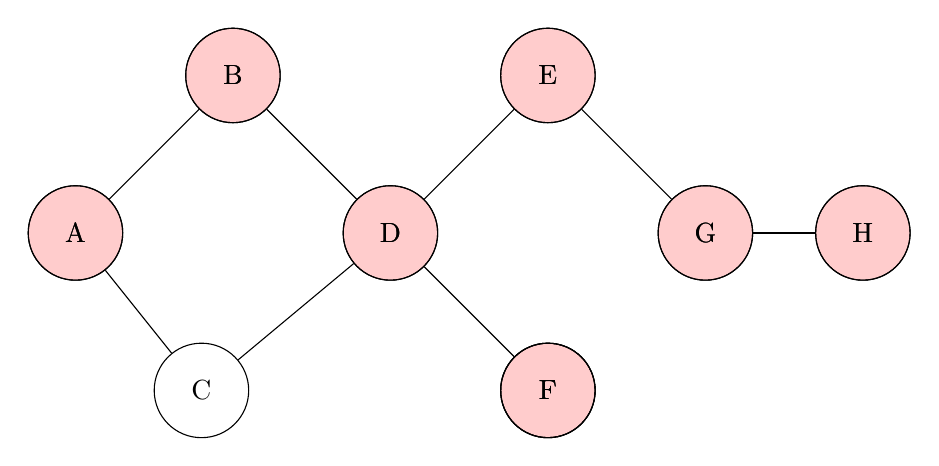
\begin{tikzpicture}
    % 探索済みノードに赤色を塗る
    \node[circle, draw, minimum size=1.2cm, fill=red!20] (A) at (-4, 0) {A};
    \node[circle, draw, minimum size=1.2cm, fill=red!20] (B) at (-2, 2) {B};
    \node[circle, draw, minimum size=1.2cm, fill=red!20] (D) at (0, 0) {D};
    \node[circle, draw, minimum size=1.2cm, fill=red!20] (E) at (2, 2) {E};
    \node[circle, draw, minimum size=1.2cm, fill=red!20] (G) at (4, 0) {G};
    \node[circle, draw, minimum size=1.2cm, fill=red!20] (F) at (2, -2) {F};
    \node[circle, draw, minimum size=1.2cm, fill=red!20] (H) at (6, 0) {H};
    \node[circle, draw, minimum size=1.2cm] (F) at (2, -2) {F};
    % ノード
    \node[circle, draw, minimum size=1.2cm] (A) at (-4, 0) {A};
    \node[circle, draw, minimum size=1.2cm] (B) at (-2, 2) {B};
    \node[circle, draw, minimum size=1.2cm] (C) at (-2.4, -2) {C};
    \node[circle, draw, minimum size=1.2cm] (D) at (0, 0) {D};
    \node[circle, draw, minimum size=1.2cm] (E) at (2, 2) {E};
    \node[circle, draw, minimum size=1.2cm] (F) at (2, -2) {F};
    \node[circle, draw, minimum size=1.2cm] (G) at (4, 0) {G};
    \node[circle, draw, minimum size=1.2cm] (H) at (6, 0) {H};

    % エッジ
    \draw (A) -- (B);
    \draw (A) -- (C);
    \draw (C) -- (D);
    \draw (B) -- (D);
    \draw (D) -- (E);
    \draw (D) -- (F);
    \draw (E) -- (G);
    \draw (G) -- (H);
  \end{tikzpicture}
\end{center}

\vspace{0.5cm}

最後にまだ探索できるAに繋がっているCの探索を行います。

\vspace{0.5cm}

\begin{center}
  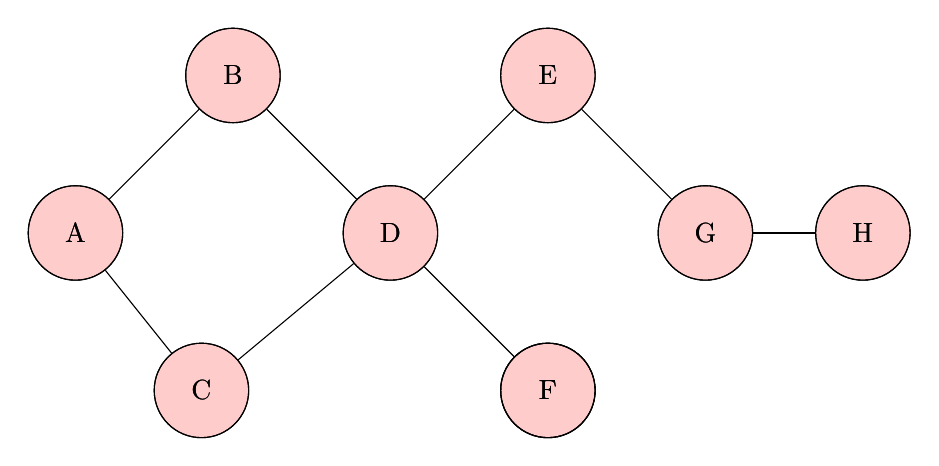
\begin{tikzpicture}
    % 探索済みノードに赤色を塗る
    \node[circle, draw, minimum size=1.2cm, fill=red!20] (A) at (-4, 0) {A};
    \node[circle, draw, minimum size=1.2cm, fill=red!20] (B) at (-2, 2) {B};
    \node[circle, draw, minimum size=1.2cm, fill=red!20] (D) at (0, 0) {D};
    \node[circle, draw, minimum size=1.2cm, fill=red!20] (E) at (2, 2) {E};
    \node[circle, draw, minimum size=1.2cm, fill=red!20] (G) at (4, 0) {G};
    \node[circle, draw, minimum size=1.2cm, fill=red!20] (F) at (2, -2) {F};
    \node[circle, draw, minimum size=1.2cm, fill=red!20] (H) at (6, 0) {H};
    \node[circle, draw, minimum size=1.2cm] (F) at (2, -2) {F};
    \node[circle, draw, minimum size=1.2cm, fill=red!20] (C) at (-2.4, -2) {C};
    % ノード
    \node[circle, draw, minimum size=1.2cm] (A) at (-4, 0) {A};
    \node[circle, draw, minimum size=1.2cm] (B) at (-2, 2) {B};
    \node[circle, draw, minimum size=1.2cm] (C) at (-2.4, -2) {C};
    \node[circle, draw, minimum size=1.2cm] (D) at (0, 0) {D};
    \node[circle, draw, minimum size=1.2cm] (E) at (2, 2) {E};
    \node[circle, draw, minimum size=1.2cm] (F) at (2, -2) {F};
    \node[circle, draw, minimum size=1.2cm] (G) at (4, 0) {G};
    \node[circle, draw, minimum size=1.2cm] (H) at (6, 0) {H};

    % エッジ
    \draw (A) -- (B);
    \draw (A) -- (C);
    \draw (C) -- (D);
    \draw (B) -- (D);
    \draw (D) -- (E);
    \draw (D) -- (F);
    \draw (E) -- (G);
    \draw (G) -- (H);
  \end{tikzpicture}
\end{center}

\vspace{0.5cm}

これでグラフの探索が終了しました。DFSは猪突猛進な探索方法で、BFSとは異なり、最短経路を求めることができません。

\subsection{DFSの実装(スタック)}
DFSの実装はスタックを用いて行います。実装のポイントは以下の通りです。

\begin{itemize}
  \item スタックを用いて、次に探索するノードを管理する
  \item 探索済みのノードを管理するために、配列を用いる
\end{itemize}

隣接リストでも隣接行列でも実装できますが、隣接リストの方が実装が簡単です。また0-indexedで実装している
ことに注意してください。DFSとの違いは、キューをスタックに変えるだけです。

\begin{lstlisting}[caption=深さ優先探索ヒープの実装, label=dfs, frame=TRBL, label={dfs}]
  from collections import deque

  def dfs(graph: list[list[int]], start: int) -> list[bool]:
      visited = [False] * len(graph)
      todo = deque()
      
      # スタート地点で初期化
      todo.append(start)
      
      while todo:
          node = todo.pop()
          visited[node] = True
          
          for next_node in graph[node]:
              if not visited[next_node]:
                  todo.append(next_node)
                  
      return visited
\end{lstlisting}
\subsection{DFSの実装(再帰)}
DFSは再帰を用いて実装することもできます。再帰を用いると、スタックを用いた実装よりも簡潔に実装することができます。

\begin{lstlisting}[caption=深さ優先探索再帰の実装, label=dfs_recursive, frame=TRBL, label={dfs_recursive}]
def dfs(graph: list[list[int]], start: int, visited: list[bool]) -> list[bool]:   
    visited[start] = True
    for next_node in graph[start]:
        if visited[next_node]:
            continue
        else:
            dfs(graph, next_node, visited)
    
    return visited
\end{lstlisting}

\newpage

\section{素集合データ構造(Union-Find木)}
Union-Find木はノードの集合の連結性を管理するデータ構造です。下の例では、AとDが同じノードにあるかを高速に判定したり、逆にAとDを連結したりする操作を
行うことができます。Union-Find木は以下の操作を行います。

\vspace{0.5cm}

\begin{itemize}
  \item Union 2つの集合を結合する
  \item Find: 2つのノードが同じ集合に属しているかを判定する
\end{itemize}

\vspace{0.5cm}

\begin{tabular}{c @{\hspace{3cm}} c @{\hspace{3cm}} c} 

  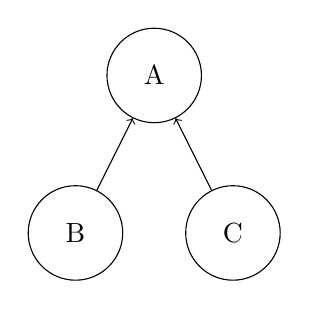
\begin{tikzpicture}
    \node[circle, draw, minimum size=1.2cm] (A) at (0, 2) {A};
    \node[circle, draw, minimum size=1.2cm] (B) at (-1, 0) {B};
    \node[circle, draw, minimum size=1.2cm] (C) at (1, 0) {C};

    \draw[<-] (A) -- (B);
    \draw[<-] (A) -- (C);
  \end{tikzpicture}
  &
  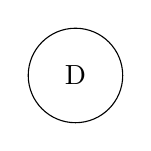
\begin{tikzpicture}
    \node[circle, draw, minimum size=1.2cm] (D) at (0, 2) {D};
  \end{tikzpicture}
  &
  % 右の木
  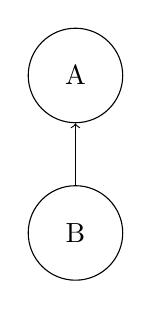
\begin{tikzpicture}
    \node[circle, draw, minimum size=1.2cm] (A) at (0, 2) {A};
    \node[circle, draw, minimum size=1.2cm] (B) at (0, 0) {B};

    \draw[->] (B) -- (A);
  \end{tikzpicture}

\end{tabular}




\begin{lstlisting}[caption=Union-Find木の実装, label=union_find, frame=TRBL, label={union_find}]
class UnionFind:
  def __init__(self, n: int) -> None:
      self.parent = [i for i in range(n)]
      self.rank = [0] * n
  
  def _root(self, node: int) -> int:
      if self.parent[node] == node:
          return node
      else:
          # 経路圧縮
          self.parent[node] = self._root(node)
          return self.parent[node]
  
  def unite(self, x: int, y: int) -> None:
      root_x = self._root(x)
      root_y = self._root(y)
      
      if root_x != root_y:
          if self.rank[root_x] < self.rank[root_y]:
              self.parent[root_x] = root_y
          else:
              self.parent[root_y] = root_x
              if self.parent[root_x] == self.parent[root_y]:
                  self.rank[root_x] += 1
  def is_same(self, x: int, y: int) -> bool:
      return self.parent[x] == self.parent[y]


\end{lstlisting}


\newpage
\section{最短経路問題}
BFSを用いた最短経路は上で紹介しましたが、今回はより効率的な最短経路問題の解法を紹介します。DFSでは重さが同じのグラフでしか最短経路を求めることができませんが、
ダイクストラ法を用いることで重さに異なる重み付きグラフでも最短経路を求めることができます。また、負の重みがあっても最短経路を求めることができるベルマン・フォード法も紹介します。

\subsection{ダイクストラ法}
ダイクストラ法を理解する上で重要な重み付きグラフの性質を紹介します。

\begin{theorembox}[経路緩和性]
  最短経路の部分経路も最短経路である


  \dotfill \\
  簡単な証明 \\
  Pを最短経路とし、その部分経路をQとする。もしもQよりも短い経路Rが存在するとすると、Rを使った経路の方がPよりも短い経路になるため、Pは最短経路ではない。
  Pが最短経路であるという過程に矛盾が生じるため、Qも最短経路である。
\end{theorembox}

具体例を挙げて説明します。以下のグラフを考えます。

\vspace{0.5cm}

\begin{center}
  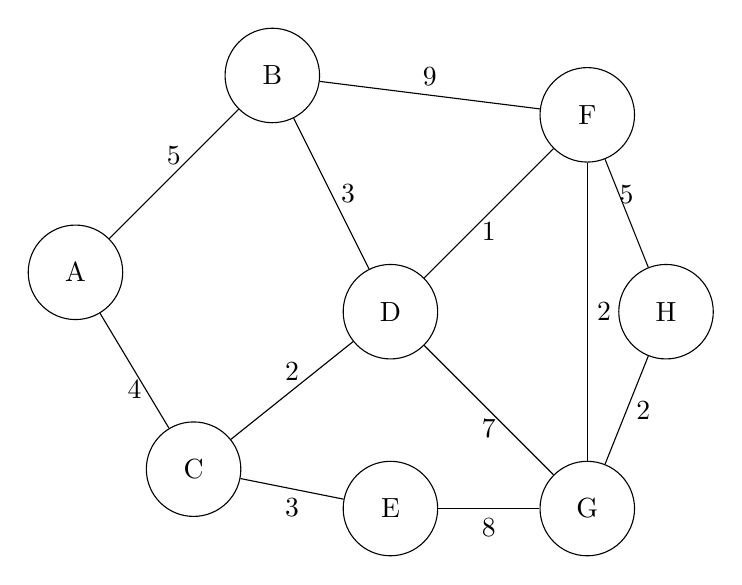
\begin{tikzpicture}
    \node[circle, draw, minimum size=1.2cm] (A) at (0, 0) {A};
    \node[circle, draw, minimum size=1.2cm] (B) at (2.5, 2.5) {B};
    \node[circle, draw, minimum size=1.2cm] (C) at (1.5, -2.5) {C};
    \node[circle, draw, minimum size=1.2cm] (D) at (4, -0.5) {D};
    \node[circle, draw, minimum size=1.2cm] (E) at (4, -3) {E};
    \node[circle, draw, minimum size=1.2cm] (F) at (6.5, 2) {F};
    \node[circle, draw, minimum size=1.2cm] (H) at (7.5, -0.5) {H};
    \node[circle, draw, minimum size=1.2cm] (G) at (6.5, -3) {G};

    \draw (A) -- node[above] {5} (B);
    \draw (A) -- node[below] {4} (C);
    \draw (C) -- node[above] {2} (D);
    \draw (B) -- node[right] {3} (D);
    \draw (B) -- node[above] {9} (F);
    \draw (F) -- node[above] {5} (H);
    \draw (C) -- node[below] {3} (E);
    \draw (E) -- node[below] {8} (G);
    \draw (D) -- node[below] {7} (G);
    \draw (D) -- node[below] {1} (F);
    \draw (G) -- node[right] {2} (H);
    \draw (F) -- node[right] {2} (G);

  \end{tikzpicture}
\end{center}

\vspace{0.5cm}

AからHまでの最短経路は以下の通りです。もしもゴールがG、F、D、Cいずれの場合でも、最短経路はA→C→D→F→G→Hの経路になります。

\vspace{0.5cm}

\begin{center}
  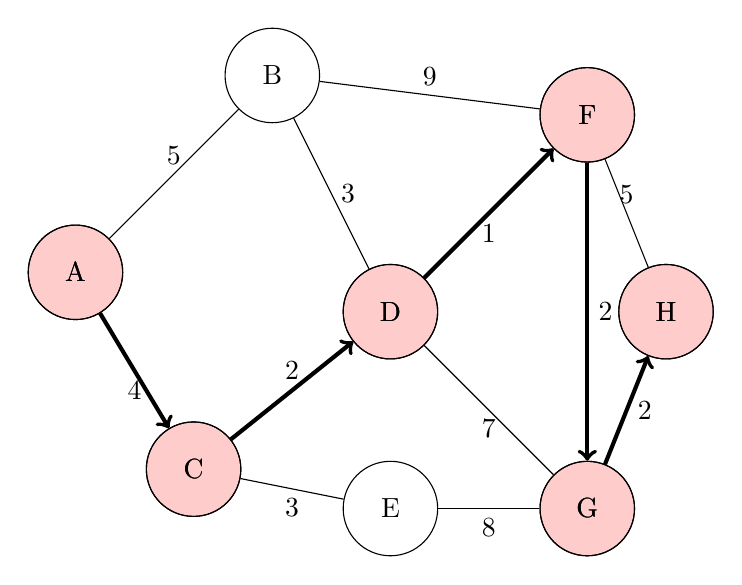
\begin{tikzpicture}
    % 最短経路に赤色を塗る
    \node[circle, draw, minimum size=1.2cm, fill=red!20] (A) at (0, 0) {A};
    \node[circle, draw, minimum size=1.2cm, fill=red!20] (C) at (1.5, -2.5) {C};
    \node[circle, draw, minimum size=1.2cm, fill=red!20] (D) at (4, -0.5) {D};
    \node[circle, draw, minimum size=1.2cm, fill=red!20] (F) at (6.5, 2) {F};
    \node[circle, draw, minimum size=1.2cm, fill=red!20] (G) at (6.5, -3) {G};
    \node[circle, draw, minimum size=1.2cm, fill=red!20] (H) at (7.5, -0.5) {H};

    \node[circle, draw, minimum size=1.2cm] (A) at (0, 0) {A};
    \node[circle, draw, minimum size=1.2cm] (B) at (2.5, 2.5) {B};
    \node[circle, draw, minimum size=1.2cm] (C) at (1.5, -2.5) {C};
    \node[circle, draw, minimum size=1.2cm] (D) at (4, -0.5) {D};
    \node[circle, draw, minimum size=1.2cm] (E) at (4, -3) {E};
    \node[circle, draw, minimum size=1.2cm] (F) at (6.5, 2) {F};
    \node[circle, draw, minimum size=1.2cm] (H) at (7.5, -0.5) {H};
    \node[circle, draw, minimum size=1.2cm] (G) at (6.5, -3) {G};

    \draw (A) -- node[above] {5} (B);
    \draw[line width=1.5pt, ->] (A) -- node[below] {4} (C);
    \draw[line width=1.5pt, ->] (C) -- node[above] {2} (D);
    \draw (B) -- node[right] {3} (D);
    \draw (B) -- node[above] {9} (F);
    \draw (F) -- node[above] {5} (H);
    \draw (C) -- node[below] {3} (E);
    \draw (E) -- node[below] {8} (G);
    \draw (D) -- node[below] {7} (G);
    \draw[line width=1.5pt, ->] (D) -- node[below] {1} (F);
    \draw[line width=1.5pt, ->]  (G) -- node[right] {2} (H);
    \draw[line width=1.5pt, ->]  (F) -- node[right] {2} (G);

  \end{tikzpicture}
\end{center}

\vspace{0.5cm}

以上の性質より、あるノードまでの最短経路を考えるときはそのノードの前のノードまでの最短経路を考えればよいことがわかります。この性質を利用したのアルゴリズムがダイクストラ法です。
ダイクストラ法は以下の手順で最短経路を求めることができます。

\begin{enumerate}
  \item まだ距離が確定していないノードのうち、最も距離が短いノード$x$を選択する
  \item ノード$x$に繋がっているノードの距離を更新する
  \item 更新が終わるとノード$x$の距離を確定する
  \item すべての頂点が確定するまで1から3を繰り返す
\end{enumerate}

距離は$\infty$、スタート地点は0で初期化します。上のグラフを例にしてダイクストラ法の例を見てみます。
最初の距離が確定していないのーどで最も距離が短いノードはAです。Aに繋がっているノードの距離を更新します。

\vspace{0.5cm}

\begin{center}
  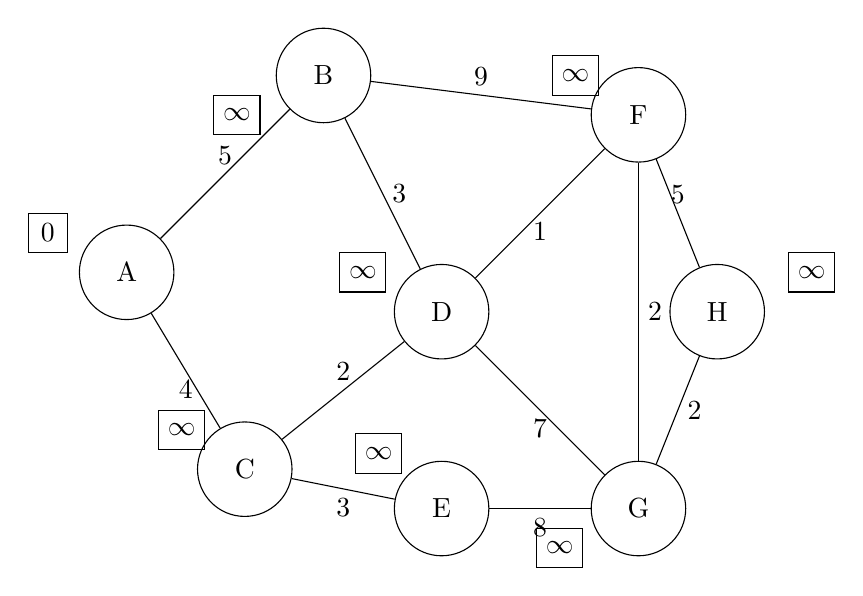
\begin{tikzpicture}
    \node[rectangle, draw, minimum size=0.5cm, xshift=-0.8cm, yshift=0.5cm] (A_label) at (-0.2, 0) {0};
    \node[rectangle, draw, minimum size=0.5cm, xshift=-0.8cm, yshift=-0.5cm] (B_label) at (2.2, 2.5) {$\infty$};
    \node[rectangle, draw, minimum size=0.5cm, xshift=-0.8cm, yshift=0.5cm] (C_label) at (1.5, -2.5) {$\infty$};
    \node[rectangle, draw, minimum size=0.5cm, xshift=-0.8cm, yshift=0.5cm] (D_label) at (3.8, -0.5) {$\infty$};
    \node[rectangle, draw, minimum size=0.5cm, xshift=-0.8cm, yshift=0.5cm] (E_label) at (4, -2.8) {$\infty$};
    \node[rectangle, draw, minimum size=0.5cm, xshift=-0.8cm, yshift=0.5cm] (F_label) at (6.5, 2) {$\infty$};
    \node[rectangle, draw, minimum size=0.5cm, xshift=-0.8cm, yshift=0.5cm] (G_label) at (6.3, -4) {$\infty$};
    \node[rectangle, draw, minimum size=0.5cm, xshift=-0.8cm, yshift=0.5cm] (H_label) at (9.5, -0.5) {$\infty$};


    \node[circle, draw, minimum size=1.2cm] (A) at (0, 0) {A};
    \node[circle, draw, minimum size=1.2cm] (B) at (2.5, 2.5) {B};
    \node[circle, draw, minimum size=1.2cm] (C) at (1.5, -2.5) {C};
    \node[circle, draw, minimum size=1.2cm] (D) at (4, -0.5) {D};
    \node[circle, draw, minimum size=1.2cm] (E) at (4, -3) {E};
    \node[circle, draw, minimum size=1.2cm] (F) at (6.5, 2) {F};
    \node[circle, draw, minimum size=1.2cm] (H) at (7.5, -0.5) {H};
    \node[circle, draw, minimum size=1.2cm] (G) at (6.5, -3) {G};

    \draw (A) -- node[above] {5} (B);
    \draw (A) -- node[below] {4} (C);
    \draw (C) -- node[above] {2} (D);
    \draw (B) -- node[right] {3} (D);
    \draw (B) -- node[above] {9} (F);
    \draw (F) -- node[above] {5} (H);
    \draw (C) -- node[below] {3} (E);
    \draw (E) -- node[below] {8} (G);
    \draw (D) -- node[below] {7} (G);
    \draw (D) -- node[below] {1} (F);
    \draw (G) -- node[right] {2} (H);
    \draw (F) -- node[right] {2} (G);

  \end{tikzpicture}
\end{center}

\vspace{0.5cm}

最初の距離が確定していないのーどで最も距離が短いノードはAです。Aに繋がっているノードの距離を更新します。
更新が終わったので、Aの距離を確定します。

\vspace{0.5cm}

\begin{center}
  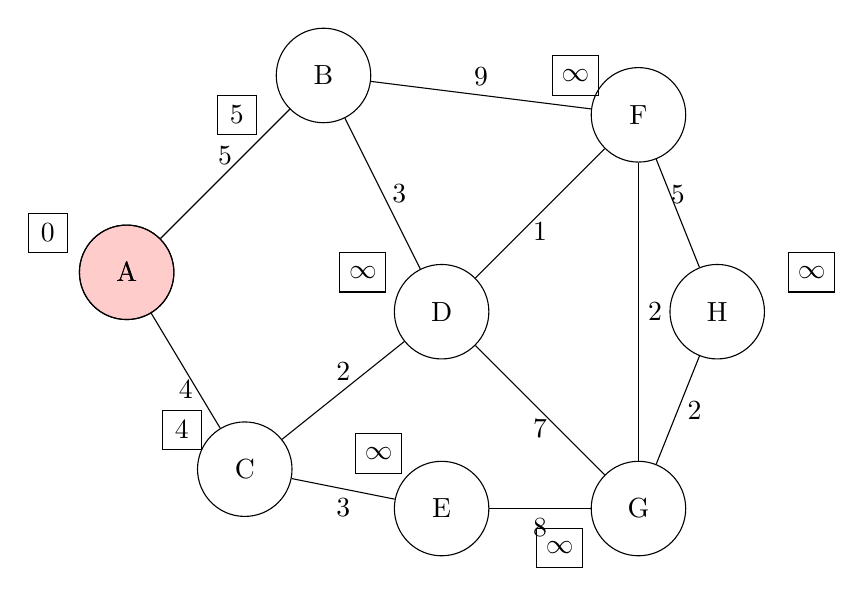
\begin{tikzpicture}
    % 確定したノードに赤色を塗る
    \node[circle, draw, minimum size=1.2cm, fill=red!20] (A) at (0, 0) {A};

    \node[rectangle, draw, minimum size=0.5cm, xshift=-0.8cm, yshift=0.5cm] (A_label) at (-0.2, 0) {0};
    \node[rectangle, draw, minimum size=0.5cm, xshift=-0.8cm, yshift=-0.5cm] (B_label) at (2.2, 2.5) {5};
    \node[rectangle, draw, minimum size=0.5cm, xshift=-0.8cm, yshift=0.5cm] (C_label) at (1.5, -2.5) {4};
    \node[rectangle, draw, minimum size=0.5cm, xshift=-0.8cm, yshift=0.5cm] (D_label) at (3.8, -0.5) {$\infty$};
    \node[rectangle, draw, minimum size=0.5cm, xshift=-0.8cm, yshift=0.5cm] (E_label) at (4, -2.8) {$\infty$};
    \node[rectangle, draw, minimum size=0.5cm, xshift=-0.8cm, yshift=0.5cm] (F_label) at (6.5, 2) {$\infty$};
    \node[rectangle, draw, minimum size=0.5cm, xshift=-0.8cm, yshift=0.5cm] (G_label) at (6.3, -4) {$\infty$};
    \node[rectangle, draw, minimum size=0.5cm, xshift=-0.8cm, yshift=0.5cm] (H_label) at (9.5, -0.5) {$\infty$};


    \node[circle, draw, minimum size=1.2cm] (A) at (0, 0) {A};
    \node[circle, draw, minimum size=1.2cm] (B) at (2.5, 2.5) {B};
    \node[circle, draw, minimum size=1.2cm] (C) at (1.5, -2.5) {C};
    \node[circle, draw, minimum size=1.2cm] (D) at (4, -0.5) {D};
    \node[circle, draw, minimum size=1.2cm] (E) at (4, -3) {E};
    \node[circle, draw, minimum size=1.2cm] (F) at (6.5, 2) {F};
    \node[circle, draw, minimum size=1.2cm] (H) at (7.5, -0.5) {H};
    \node[circle, draw, minimum size=1.2cm] (G) at (6.5, -3) {G};

    \draw (A) -- node[above] {5} (B);
    \draw (A) -- node[below] {4} (C);
    \draw (C) -- node[above] {2} (D);
    \draw (B) -- node[right] {3} (D);
    \draw (B) -- node[above] {9} (F);
    \draw (F) -- node[above] {5} (H);
    \draw (C) -- node[below] {3} (E);
    \draw (E) -- node[below] {8} (G);
    \draw (D) -- node[below] {7} (G);
    \draw (D) -- node[below] {1} (F);
    \draw (G) -- node[right] {2} (H);
    \draw (F) -- node[right] {2} (G);

  \end{tikzpicture}
\end{center}

\vspace{0.5cm}

次に距離が確定していないノードで最も距離が短いノードを選択します。今回はCです。Cに繋がっているノードの距離を更新します。
Cに繋がっているノードを更新したら、Cの距離を確定します。

\vspace{0.5cm}

\begin{center}
  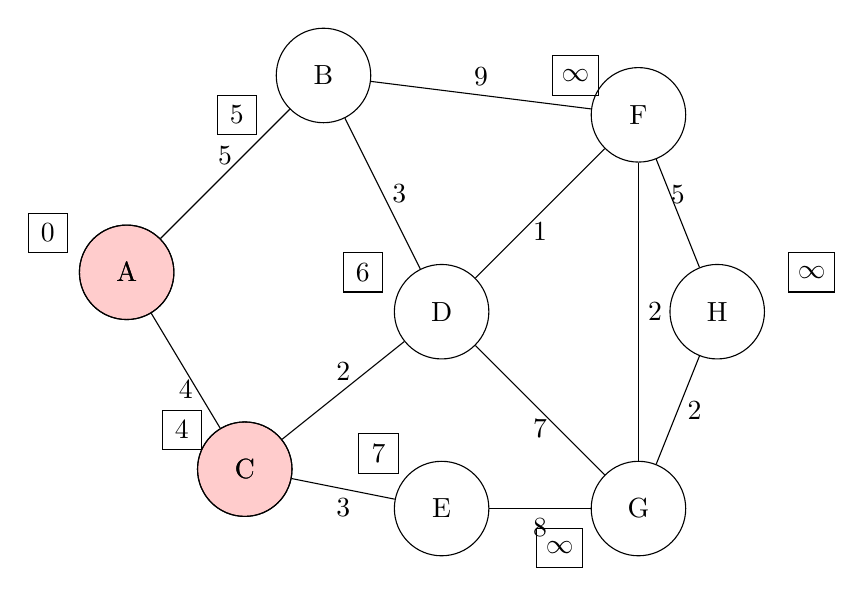
\begin{tikzpicture}
    % 確定したノードに赤色を塗る
    \node[circle, draw, minimum size=1.2cm, fill=red!20] (A) at (0, 0) {A};
    \node[circle, draw, minimum size=1.2cm, fill=red!20] (C) at (1.5, -2.5) {C};

    \node[rectangle, draw, minimum size=0.5cm, xshift=-0.8cm, yshift=0.5cm] (A_label) at (-0.2, 0) {0};
    \node[rectangle, draw, minimum size=0.5cm, xshift=-0.8cm, yshift=-0.5cm] (B_label) at (2.2, 2.5) {5};
    \node[rectangle, draw, minimum size=0.5cm, xshift=-0.8cm, yshift=0.5cm] (C_label) at (1.5, -2.5) {4};
    \node[rectangle, draw, minimum size=0.5cm, xshift=-0.8cm, yshift=0.5cm] (D_label) at (3.8, -0.5) {6};
    \node[rectangle, draw, minimum size=0.5cm, xshift=-0.8cm, yshift=0.5cm] (E_label) at (4, -2.8) {7};
    \node[rectangle, draw, minimum size=0.5cm, xshift=-0.8cm, yshift=0.5cm] (F_label) at (6.5, 2) {$\infty$};
    \node[rectangle, draw, minimum size=0.5cm, xshift=-0.8cm, yshift=0.5cm] (G_label) at (6.3, -4) {$\infty$};
    \node[rectangle, draw, minimum size=0.5cm, xshift=-0.8cm, yshift=0.5cm] (H_label) at (9.5, -0.5) {$\infty$};


    \node[circle, draw, minimum size=1.2cm] (A) at (0, 0) {A};
    \node[circle, draw, minimum size=1.2cm] (B) at (2.5, 2.5) {B};
    \node[circle, draw, minimum size=1.2cm] (C) at (1.5, -2.5) {C};
    \node[circle, draw, minimum size=1.2cm] (D) at (4, -0.5) {D};
    \node[circle, draw, minimum size=1.2cm] (E) at (4, -3) {E};
    \node[circle, draw, minimum size=1.2cm] (F) at (6.5, 2) {F};
    \node[circle, draw, minimum size=1.2cm] (H) at (7.5, -0.5) {H};
    \node[circle, draw, minimum size=1.2cm] (G) at (6.5, -3) {G};

    \draw (A) -- node[above] {5} (B);
    \draw (A) -- node[below] {4} (C);
    \draw (C) -- node[above] {2} (D);
    \draw (B) -- node[right] {3} (D);
    \draw (B) -- node[above] {9} (F);
    \draw (F) -- node[above] {5} (H);
    \draw (C) -- node[below] {3} (E);
    \draw (E) -- node[below] {8} (G);
    \draw (D) -- node[below] {7} (G);
    \draw (D) -- node[below] {1} (F);
    \draw (G) -- node[right] {2} (H);
    \draw (F) -- node[right] {2} (G);

  \end{tikzpicture}
\end{center}

\vspace{0.5cm}

次に距離が確定していないノードで最も距離が短いノードを選択します。今回はBです。Bに繋がっているノードの距離を更新します。
Dに関しては、すでにわかっている経路の方が短いので更新しません。Bの距離を確定します。

\vspace{0.5cm}

\begin{center}
  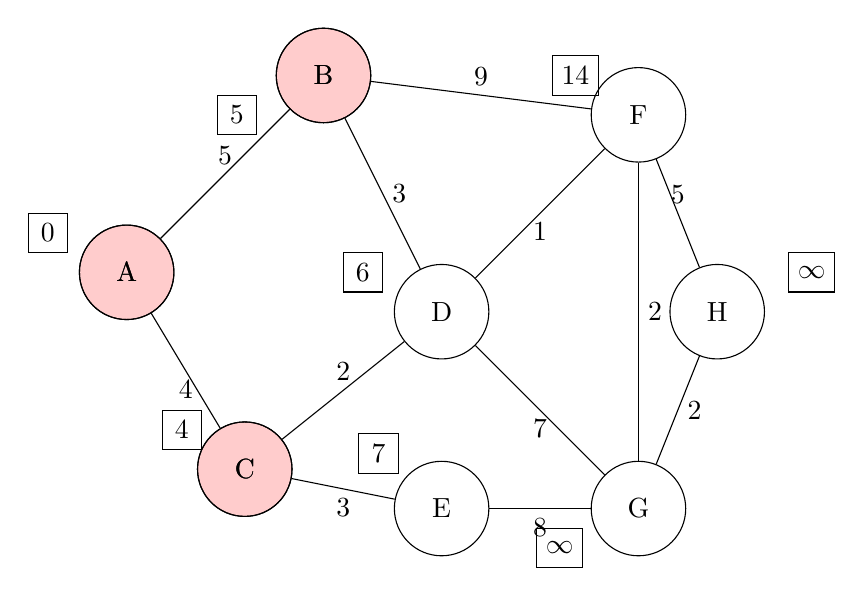
\begin{tikzpicture}
    % 確定したノードに赤色を塗る
    \node[circle, draw, minimum size=1.2cm, fill=red!20] (A) at (0, 0) {A};
    \node[circle, draw, minimum size=1.2cm, fill=red!20] (C) at (1.5, -2.5) {C};
    \node[circle, draw, minimum size=1.2cm, fill=red!20] (B) at (2.5, 2.5) {B};

    \node[rectangle, draw, minimum size=0.5cm, xshift=-0.8cm, yshift=0.5cm] (A_label) at (-0.2, 0) {0};
    \node[rectangle, draw, minimum size=0.5cm, xshift=-0.8cm, yshift=-0.5cm] (B_label) at (2.2, 2.5) {5};
    \node[rectangle, draw, minimum size=0.5cm, xshift=-0.8cm, yshift=0.5cm] (C_label) at (1.5, -2.5) {4};
    \node[rectangle, draw, minimum size=0.5cm, xshift=-0.8cm, yshift=0.5cm] (D_label) at (3.8, -0.5) {6};
    \node[rectangle, draw, minimum size=0.5cm, xshift=-0.8cm, yshift=0.5cm] (E_label) at (4, -2.8) {7};
    \node[rectangle, draw, minimum size=0.5cm, xshift=-0.8cm, yshift=0.5cm] (F_label) at (6.5, 2) {14};
    \node[rectangle, draw, minimum size=0.5cm, xshift=-0.8cm, yshift=0.5cm] (G_label) at (6.3, -4) {$\infty$};
    \node[rectangle, draw, minimum size=0.5cm, xshift=-0.8cm, yshift=0.5cm] (H_label) at (9.5, -0.5) {$\infty$};


    \node[circle, draw, minimum size=1.2cm] (A) at (0, 0) {A};
    \node[circle, draw, minimum size=1.2cm] (B) at (2.5, 2.5) {B};
    \node[circle, draw, minimum size=1.2cm] (C) at (1.5, -2.5) {C};
    \node[circle, draw, minimum size=1.2cm] (D) at (4, -0.5) {D};
    \node[circle, draw, minimum size=1.2cm] (E) at (4, -3) {E};
    \node[circle, draw, minimum size=1.2cm] (F) at (6.5, 2) {F};
    \node[circle, draw, minimum size=1.2cm] (H) at (7.5, -0.5) {H};
    \node[circle, draw, minimum size=1.2cm] (G) at (6.5, -3) {G};

    \draw (A) -- node[above] {5} (B);
    \draw (A) -- node[below] {4} (C);
    \draw (C) -- node[above] {2} (D);
    \draw (B) -- node[right] {3} (D);
    \draw (B) -- node[above] {9} (F);
    \draw (F) -- node[above] {5} (H);
    \draw (C) -- node[below] {3} (E);
    \draw (E) -- node[below] {8} (G);
    \draw (D) -- node[below] {7} (G);
    \draw (D) -- node[below] {1} (F);
    \draw (G) -- node[right] {2} (H);
    \draw (F) -- node[right] {2} (G);

  \end{tikzpicture}
\end{center}

\vspace{0.5cm}

以下同様に更新すると、最終的に以下のような結果になります。

\vspace{0.5cm}

\begin{center}
  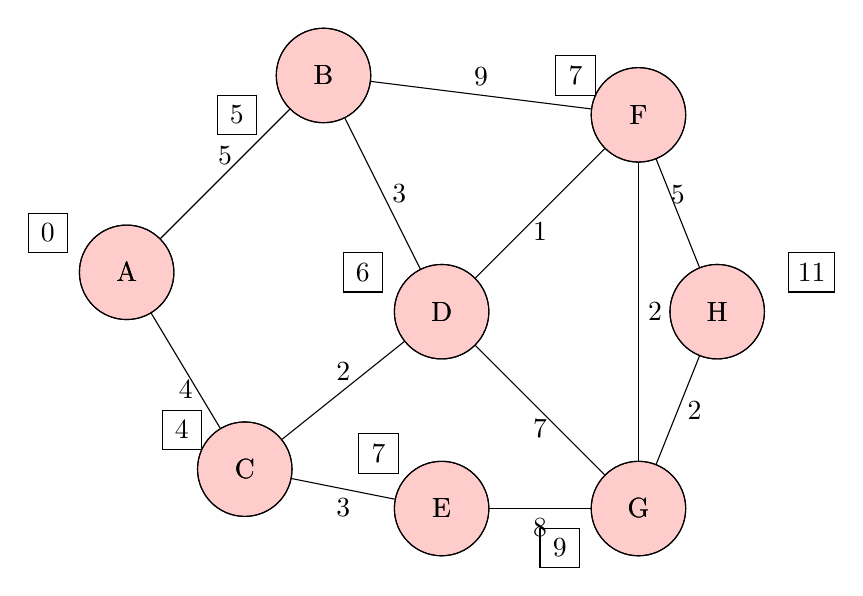
\begin{tikzpicture}
    % 確定したノードに赤色を塗る
    \node[circle, draw, minimum size=1.2cm, fill=red!20] (A) at (0, 0) {A};
    \node[circle, draw, minimum size=1.2cm, fill=red!20] (C) at (1.5, -2.5) {C};
    \node[circle, draw, minimum size=1.2cm, fill=red!20] (B) at (2.5, 2.5) {B};
    \node[circle, draw, minimum size=1.2cm, fill=red!20] (D) at (4, -0.5) {D};
    \node[circle, draw, minimum size=1.2cm, fill=red!20] (E) at (4, -3) {E};
    \node[circle, draw, minimum size=1.2cm, fill=red!20] (F) at (6.5, 2) {F};
    \node[circle, draw, minimum size=1.2cm, fill=red!20] (G) at (6.5, -3) {G};
    \node[circle, draw, minimum size=1.2cm, fill=red!20] (H) at (7.5, -0.5) {H};


    \node[rectangle, draw, minimum size=0.5cm, xshift=-0.8cm, yshift=0.5cm] (A_label) at (-0.2, 0) {0};
    \node[rectangle, draw, minimum size=0.5cm, xshift=-0.8cm, yshift=-0.5cm] (B_label) at (2.2, 2.5) {5};
    \node[rectangle, draw, minimum size=0.5cm, xshift=-0.8cm, yshift=0.5cm] (C_label) at (1.5, -2.5) {4};
    \node[rectangle, draw, minimum size=0.5cm, xshift=-0.8cm, yshift=0.5cm] (D_label) at (3.8, -0.5) {6};
    \node[rectangle, draw, minimum size=0.5cm, xshift=-0.8cm, yshift=0.5cm] (E_label) at (4, -2.8) {7};
    \node[rectangle, draw, minimum size=0.5cm, xshift=-0.8cm, yshift=0.5cm] (F_label) at (6.5, 2) {7};
    \node[rectangle, draw, minimum size=0.5cm, xshift=-0.8cm, yshift=0.5cm] (G_label) at (6.3, -4) {9};
    \node[rectangle, draw, minimum size=0.5cm, xshift=-0.8cm, yshift=0.5cm] (H_label) at (9.5, -0.5) {11};


    \node[circle, draw, minimum size=1.2cm] (A) at (0, 0) {A};
    \node[circle, draw, minimum size=1.2cm] (B) at (2.5, 2.5) {B};
    \node[circle, draw, minimum size=1.2cm] (C) at (1.5, -2.5) {C};
    \node[circle, draw, minimum size=1.2cm] (D) at (4, -0.5) {D};
    \node[circle, draw, minimum size=1.2cm] (E) at (4, -3) {E};
    \node[circle, draw, minimum size=1.2cm] (F) at (6.5, 2) {F};
    \node[circle, draw, minimum size=1.2cm] (H) at (7.5, -0.5) {H};
    \node[circle, draw, minimum size=1.2cm] (G) at (6.5, -3) {G};

    \draw (A) -- node[above] {5} (B);
    \draw (A) -- node[below] {4} (C);
    \draw (C) -- node[above] {2} (D);
    \draw (B) -- node[right] {3} (D);
    \draw (B) -- node[above] {9} (F);
    \draw (F) -- node[above] {5} (H);
    \draw (C) -- node[below] {3} (E);
    \draw (E) -- node[below] {8} (G);
    \draw (D) -- node[below] {7} (G);
    \draw (D) -- node[below] {1} (F);
    \draw (G) -- node[right] {2} (H);
    \draw (F) -- node[right] {2} (G);

  \end{tikzpicture}
\end{center}

\vspace{0.5cm}

\subsubsection{ダイクストラ法の実装}
ダイクストラ法はとてもシンプルなアルゴリズムです。ダイクストラ法の実装のポイントは以下の通りです。

\begin{itemize}
  \item 最短距離を格納する配列を用意する
  \item まだ確定していないノードのうち、最も距離が短いノードを選択する。最も短いノードを$O(\log n)$で取得するためにヒープを使う
  \item 選択したノードに繋がっているノードの距離を前回の距離と比較して更新する
  \item すべてのノードが確定するまで繰り返す
\end{itemize}

Pythonの標準ライブラリのヒープはtupleなどを渡すindexが早い要素から比較してくれるので、ダイクストラ法の実装に適しています。
(移動距離、ノード)のtupleでヒープに追加することで、最短距離が短いノードを取得することができます。もちろん自分で実装したヒープを使っても問題ありません。

与えられる重み付きグラフは(終点、重み)の形式で隣接リストで与えられるとします。以下にダイクストラ法の実装を示します。
\begin{lstlisting}[caption=ダイクストラ法の実装, label=dijkstra, frame=TRBL, label={dijkstra}]
from heapq import heappop, heappush

def dijkstra(graph: list[list[int]], start: int) -> list[int]:
      done = [False] * len(graph)
      dist = [1 << 60] * len(graph)
      todo = []
      
      # 初期化
      dist[start] = 0
      heappush(todo, (dist[start], 0))
      
      while todo:
          distance, node = heappop(todo)
          if done[node]:
              continue
          
          # 更新
          for connected_node, weight in graph[node]:
              if distance + weight < dist[connected_node]:
                  dist[connected_node] = distance + weight
                  heappush(todo, (dist[connected_node], connected_node))
          
          done[node] = True
      
      return dist
                  
\end{lstlisting}

\newpage

\subsection{ベルマン・フォード法}
ベルマン・フォード法はダイクストラ法と異なり、負の重みを持つ辺があっても機能する単一始点全点間最短路を求めるアルゴリズムです。負の閉路の検出も可能です。
ダイクストラ法とは違って最短距離の選択を行わずに、毎回すべての辺を更新します。

ベルマン・フォード法のアルゴリズムを例を使って説明します。以下のグラフを例に考えます。概要はダイクストラ法とあまり変わりません。ただし、
グラフの情報が(始点、終点、重み)のlistで与えられるとします。例えば、(A, B, 5)はAからBへでている重みが5のノードであることを示します。

すべて列挙すると、以下の様になります。

\begin{equation*}
  \begin{aligned}
    \text{edges} =
    &(A, B, 5), (B, C, -4), (C, A, -3), (C, D, 2), (B, D, 3), (B, F, 9), (F, H, 5), \\
    &(C, E, 3), (E, G, 8), (D, G, 7), (D, F, 1), (G, H, 2), (F, G, 2)
  \end{aligned}
\end{equation*}

初期化として始点の距離は0, それ以外は$\infty$とします。ベルマン・フォード法は以下のアルゴリズムに従っています。

\begin{enumerate}
  \item edgesをすべて列挙し、始点から終点への重みを更新する
  \item 1をV - 1回繰り返す(Vはノードの数)
\end{enumerate}

V-1回の更新で、最短距離が確定します。もし、V回目にも更新がある場合は負の閉路が存在することになります。最短経路を求めるのにV - 1回の更新で十分な理由は、
経路緩和性によって開始地点から終点が最も遠い場合でも、V - 1回の更新で確定するからです。

\vspace{0.5cm}
\begin{center}
  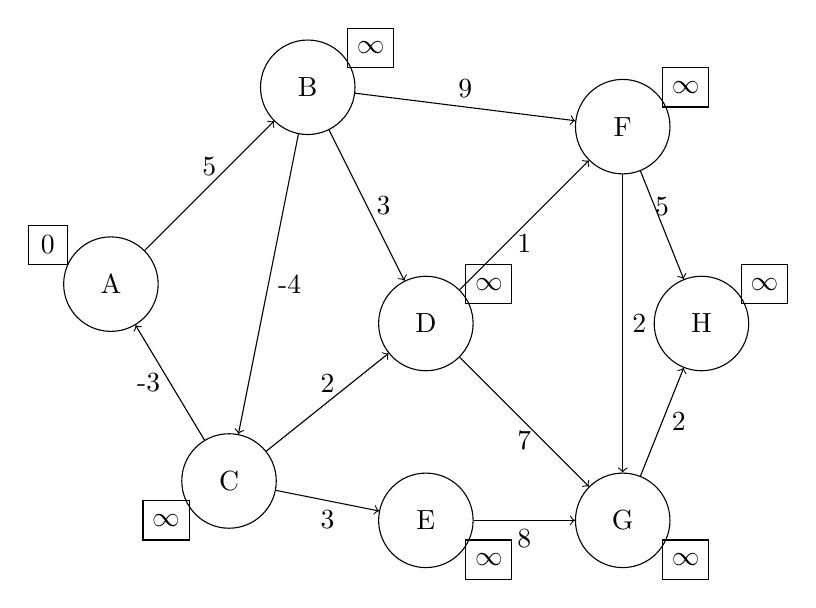
\begin{tikzpicture}
    % ノードの定義
    \node[circle, draw, minimum size=1.2cm] (A) at (0, 0) {A};
    \node[circle, draw, minimum size=1.2cm] (B) at (2.5, 2.5) {B};
    \node[circle, draw, minimum size=1.2cm] (C) at (1.5, -2.5) {C};
    \node[circle, draw, minimum size=1.2cm] (D) at (4, -0.5) {D};
    \node[circle, draw, minimum size=1.2cm] (E) at (4, -3) {E};
    \node[circle, draw, minimum size=1.2cm] (F) at (6.5, 2) {F};
    \node[circle, draw, minimum size=1.2cm] (H) at (7.5, -0.5) {H};
    \node[circle, draw, minimum size=1.2cm] (G) at (6.5, -3) {G};

    % distを表示する小さな四角を追加
    \node[rectangle, draw, minimum size=0.5cm, xshift=-0.8cm, yshift=0.5cm] at (A) {0};
    \node[rectangle, draw, minimum size=0.5cm, xshift=0.8cm, yshift=0.5cm] at (B) {$\infty$};
    \node[rectangle, draw, minimum size=0.5cm, xshift=-0.8cm, yshift=-0.5cm] at (C) {$\infty$};
    \node[rectangle, draw, minimum size=0.5cm, xshift=0.8cm, yshift=0.5cm] at (D) {$\infty$};
    \node[rectangle, draw, minimum size=0.5cm, xshift=0.8cm, yshift=-0.5cm] at (E) {$\infty$};
    \node[rectangle, draw, minimum size=0.5cm, xshift=0.8cm, yshift=0.5cm] at (F) {$\infty$};
    \node[rectangle, draw, minimum size=0.5cm, xshift=0.8cm, yshift=-0.5cm] at (G) {$\infty$};
    \node[rectangle, draw, minimum size=0.5cm, xshift=0.8cm, yshift=0.5cm] at (H) {$\infty$};

    % エッジの定義(有向グラフ)
    \draw[->] (A) -- node[above] {5} (B);
    \draw[->] (B) -- node[right] {-4} (C);
    \draw[->] (C) -- node[left] {-3} (A); % 負の閉路を形成するエッジ
    \draw[->] (C) -- node[above] {2} (D);
    \draw[->] (B) -- node[right] {3} (D);
    \draw[->] (B) -- node[above] {9} (F);
    \draw[->] (F) -- node[above] {5} (H);
    \draw[->] (C) -- node[below] {3} (E);
    \draw[->] (E) -- node[below] {8} (G);
    \draw[->] (D) -- node[below] {7} (G);
    \draw[->] (D) -- node[below] {1} (F);
    \draw[->] (G) -- node[right] {2} (H);
    \draw[->] (F) -- node[right] {2} (G);
  \end{tikzpicture}
\end{center}

\vspace{0.5cm}

ベルマン・フォード法の流れを確認します。最初はAと繋がっているBが更新されます。他のノードもedgesをすべて列挙して更新を図りますが、
$\infty +$有限の値と考えるため、更新されないとみなすことができます。
\vspace{0.5cm}
\begin{center}
  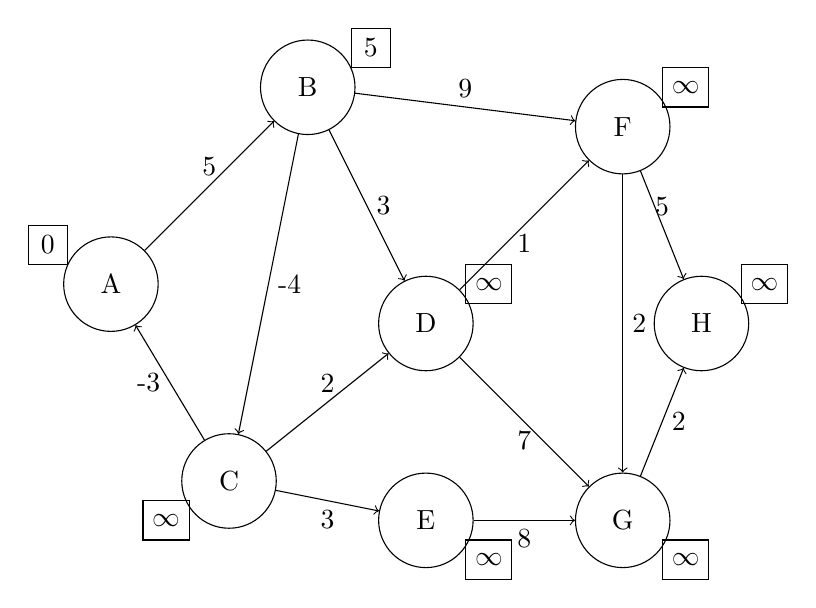
\begin{tikzpicture}
    % ノードの定義
    \node[circle, draw, minimum size=1.2cm] (A) at (0, 0) {A};
    \node[circle, draw, minimum size=1.2cm] (B) at (2.5, 2.5) {B};
    \node[circle, draw, minimum size=1.2cm] (C) at (1.5, -2.5) {C};
    \node[circle, draw, minimum size=1.2cm] (D) at (4, -0.5) {D};
    \node[circle, draw, minimum size=1.2cm] (E) at (4, -3) {E};
    \node[circle, draw, minimum size=1.2cm] (F) at (6.5, 2) {F};
    \node[circle, draw, minimum size=1.2cm] (H) at (7.5, -0.5) {H};
    \node[circle, draw, minimum size=1.2cm] (G) at (6.5, -3) {G};

    % distを表示する小さな四角を追加
    \node[rectangle, draw, minimum size=0.5cm, xshift=-0.8cm, yshift=0.5cm] at (A) {0};
    \node[rectangle, draw, minimum size=0.5cm, xshift=0.8cm, yshift=0.5cm] at (B) {5};
    \node[rectangle, draw, minimum size=0.5cm, xshift=-0.8cm, yshift=-0.5cm] at (C) {$\infty$};
    \node[rectangle, draw, minimum size=0.5cm, xshift=0.8cm, yshift=0.5cm] at (D) {$\infty$};
    \node[rectangle, draw, minimum size=0.5cm, xshift=0.8cm, yshift=-0.5cm] at (E) {$\infty$};
    \node[rectangle, draw, minimum size=0.5cm, xshift=0.8cm, yshift=0.5cm] at (F) {$\infty$};
    \node[rectangle, draw, minimum size=0.5cm, xshift=0.8cm, yshift=-0.5cm] at (G) {$\infty$};
    \node[rectangle, draw, minimum size=0.5cm, xshift=0.8cm, yshift=0.5cm] at (H) {$\infty$};

    % エッジの定義(有向グラフ)
    \draw[->] (A) -- node[above] {5} (B);
    \draw[->] (B) -- node[right] {-4} (C);
    \draw[->] (C) -- node[left] {-3} (A); % 負の閉路を形成するエッジ
    \draw[->] (C) -- node[above] {2} (D);
    \draw[->] (B) -- node[right] {3} (D);
    \draw[->] (B) -- node[above] {9} (F);
    \draw[->] (F) -- node[above] {5} (H);
    \draw[->] (C) -- node[below] {3} (E);
    \draw[->] (E) -- node[below] {8} (G);
    \draw[->] (D) -- node[below] {7} (G);
    \draw[->] (D) -- node[below] {1} (F);
    \draw[->] (G) -- node[right] {2} (H);
    \draw[->] (F) -- node[right] {2} (G);
  \end{tikzpicture}
\end{center}

\vspace{0.5cm}
2回目の更新です。

\vspace{0.5cm}
\begin{center}
  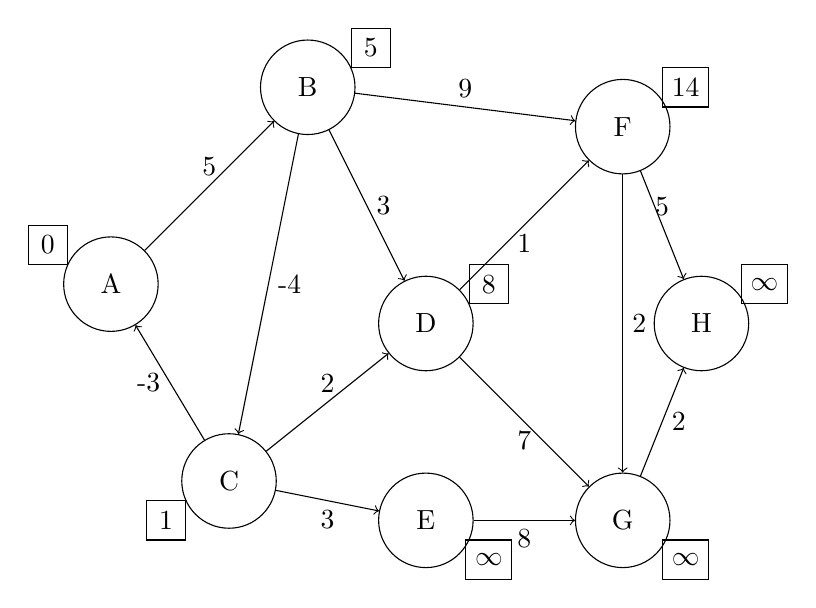
\begin{tikzpicture}
    % ノードの定義
    \node[circle, draw, minimum size=1.2cm] (A) at (0, 0) {A};
    \node[circle, draw, minimum size=1.2cm] (B) at (2.5, 2.5) {B};
    \node[circle, draw, minimum size=1.2cm] (C) at (1.5, -2.5) {C};
    \node[circle, draw, minimum size=1.2cm] (D) at (4, -0.5) {D};
    \node[circle, draw, minimum size=1.2cm] (E) at (4, -3) {E};
    \node[circle, draw, minimum size=1.2cm] (F) at (6.5, 2) {F};
    \node[circle, draw, minimum size=1.2cm] (H) at (7.5, -0.5) {H};
    \node[circle, draw, minimum size=1.2cm] (G) at (6.5, -3) {G};

    % distを表示する小さな四角を追加
    \node[rectangle, draw, minimum size=0.5cm, xshift=-0.8cm, yshift=0.5cm] at (A) {0};
    \node[rectangle, draw, minimum size=0.5cm, xshift=0.8cm, yshift=0.5cm] at (B) {5};
    \node[rectangle, draw, minimum size=0.5cm, xshift=-0.8cm, yshift=-0.5cm] at (C) {1};
    \node[rectangle, draw, minimum size=0.5cm, xshift=0.8cm, yshift=0.5cm] at (D) {8};
    \node[rectangle, draw, minimum size=0.5cm, xshift=0.8cm, yshift=-0.5cm] at (E) {$\infty$};
    \node[rectangle, draw, minimum size=0.5cm, xshift=0.8cm, yshift=0.5cm] at (F) {14};
    \node[rectangle, draw, minimum size=0.5cm, xshift=0.8cm, yshift=-0.5cm] at (G) {$\infty$};
    \node[rectangle, draw, minimum size=0.5cm, xshift=0.8cm, yshift=0.5cm] at (H) {$\infty$};

    % エッジの定義(有向グラフ)
    \draw[->] (A) -- node[above] {5} (B);
    \draw[->] (B) -- node[right] {-4} (C);
    \draw[->] (C) -- node[left] {-3} (A); % 負の閉路を形成するエッジ
    \draw[->] (C) -- node[above] {2} (D);
    \draw[->] (B) -- node[right] {3} (D);
    \draw[->] (B) -- node[above] {9} (F);
    \draw[->] (F) -- node[above] {5} (H);
    \draw[->] (C) -- node[below] {3} (E);
    \draw[->] (E) -- node[below] {8} (G);
    \draw[->] (D) -- node[below] {7} (G);
    \draw[->] (D) -- node[below] {1} (F);
    \draw[->] (G) -- node[right] {2} (H);
    \draw[->] (F) -- node[right] {2} (G);
  \end{tikzpicture}
\end{center}

\vspace{0.5cm}

以下のように更新を繰り返すと、最終的に以下のような結果になります。

\begin{lstlisting}[caption=ベルマン・フォード法の実装, label=berman, frame=TRBL, label={berman}]
def bellman_ford(v: int, edges: list[tuple[int, int, int]]) -> list[int] | int:
  # 初期化
  dist = [1 << 60] * v
  dist[0] = 0

  for _ in range(v - 1):
      for start, end, weight in edges:
          if dist[start] != 1 << 60 and dist[start] + weight < dist[end]:
              dist[end] = dist[start] + weight
  
  # 一度v-1回更新した後に負の閉路を検出
  for start, end, weight in edges:
      if dist[start] != 1 << 60 and dist[start] + weight < dist[end]:
          return -1  

  return dist
\end{lstlisting}

\newpage

\subsection{SPFA(Shortest Path Faster Algorithm)}
SPFAはベルマン・フォード法を高速化したアルゴリズムです。基本はベルマン・フォード法と同じですが、毎回すべての辺をチェックすること
防ぐ工夫がされています。あるノード$x$が更新されなければ、そのノードに繋がっている他のノードの距離も更新されません。実装上は
更新が必要なノードが出てきたらそれをqueueに入れ、queueがからになるまで処理を続けます。

SPFA実装の実装は以下の様になります。

\begin{lstlisting}[caption=SPFAの実装, label=spfa, frame=TRBL, label={spfa}]
from collections import deque

def spfa(v: int, edges: list[list[tuple[int, int]]]):
      inf = 1 << 60
      dist = [inf] * v
      dist[0] = 0
      
      node_to_check = deque()
      in_queue = [False] * v
      
      while node_to_check:
          current_node = node_to_check.popleft()
          in_queue[current_node] = False
          
          for end, weight in edges[current_node]:
              if dist[current_node] + weight < dist[end]:
                  dist[end] = dist[current_node] + weight 
              
              if not in_queue[end]:
                  in_queue[end] = True
                  node_to_check.append(end)
      
      return dist
\end{lstlisting}

\newpage

\subsection{ワーシャルフロイド法}
\begin{lstlisting}[caption=ワーシャルフロイド法の実装, label=warshall, frame=TRBL, label={warshall}]
def warshall_floyd(n: int, dist: list[list[int]]):
  for i in range(n):
      for j in range(n):
          for k in range(n):
              dist[j][k] = min(dist[j][k], dist[j][i] + dist[i][k])
\end{lstlisting}


\newpage

\section{最小全域木}
\textbf{全域木}とは、すべてのノードが繋がっている木のことをいいます。また\textbf{最小全域木}とは、全域木の中で重さが最小になるもののことをいいます。

\vspace{0.5cm}

\begin{center}
  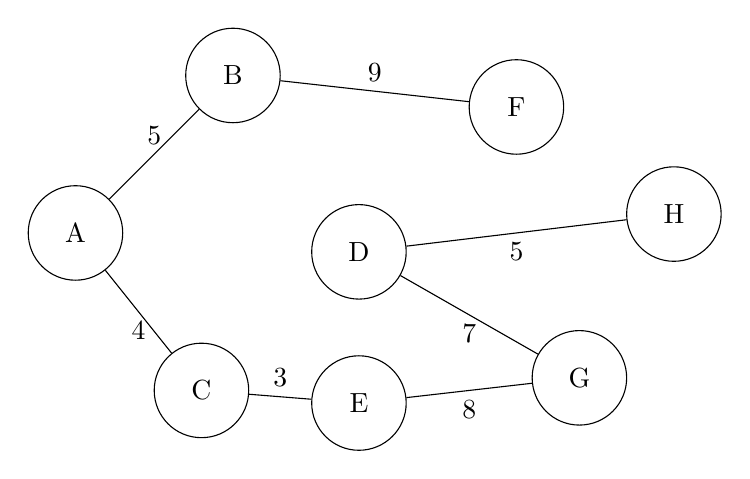
\begin{tikzpicture}[scale=0.8]
    \node[circle, draw, minimum size=1.2cm] (A) at (0, 0) {A};
    \node[circle, draw, minimum size=1.2cm] (B) at (2.5, 2.5) {B};
    \node[circle, draw, minimum size=1.2cm] (C) at (2.0, -2.5) {C};
    \node[circle, draw, minimum size=1.2cm] (D) at (4.5, -0.3) {D};
    \node[circle, draw, minimum size=1.2cm] (E) at (4.5, -2.7) {E};
    \node[circle, draw, minimum size=1.2cm] (F) at (7.0, 2.0) {F};
    \node[circle, draw, minimum size=1.2cm] (G) at (8.0, -2.3) {G};
    \node[circle, draw, minimum size=1.2cm] (H) at (9.5, 0.3) {H};

    % エッジを引く
    \draw (A) -- node[above] {5} (B);
    \draw (A) -- node[below] {4} (C);
    \draw (C) -- node[above] {3} (E);
    \draw (B) -- node[above] {9} (F);
    \draw (E) -- node[below] {8} (G);
    \draw (G) -- node[below] {7} (D);
    \draw (D) -- node[below] {5} (H);
  \end{tikzpicture}
\end{center}

\vspace{0.5cm}

最小全域木を求めるには、辺ベースのアプローチとノードベースのアプローチの2種類があります。それぞれ\textbf{クラスカル法}、\textbf{プリム法}と
呼ばれています。

\subsection{クラスカル法}
クラスカル法は、存在する辺を重さが小さい順に並べて入れていき、閉路ができないことが確認できた場合は追加し、すべての辺をチェックし終えたら終了するアルゴリズムです。
以下のアルゴリズムに従っています。

\begin{enumerate}
  \item すべての辺を重さの小さい順にソート
  \item 重さの最も小さい辺を選ぶ
  \item 今までに選んだ辺から構成される木に2で選んだ辺を追加した時に、閉路が生まれないことを確認する。閉路が新しくできないならこの辺を追加する
  \item すべての辺をチェックし終えるまで2から3を繰り返す
\end{enumerate}

\begin{center}
  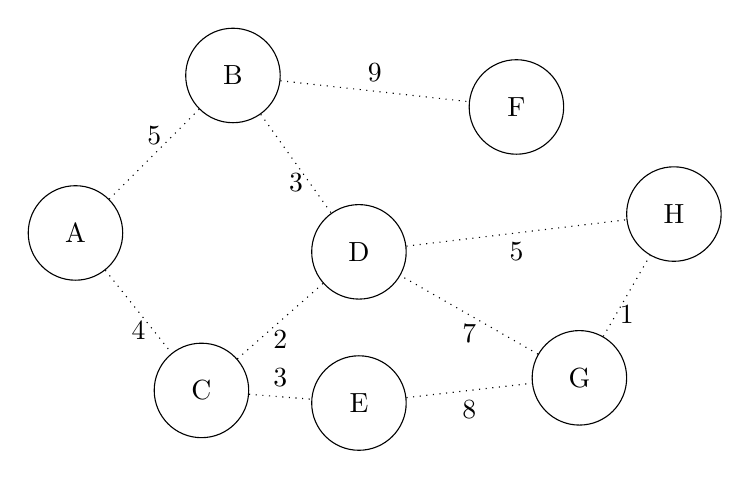
\begin{tikzpicture}[scale=0.8]
    \node[circle, draw, minimum size=1.2cm] (A) at (0, 0) {A};
    \node[circle, draw, minimum size=1.2cm] (B) at (2.5, 2.5) {B};
    \node[circle, draw, minimum size=1.2cm] (C) at (2.0, -2.5) {C};
    \node[circle, draw, minimum size=1.2cm] (D) at (4.5, -0.3) {D};
    \node[circle, draw, minimum size=1.2cm] (E) at (4.5, -2.7) {E};
    \node[circle, draw, minimum size=1.2cm] (F) at (7.0, 2.0) {F};
    \node[circle, draw, minimum size=1.2cm] (G) at (8.0, -2.3) {G};
    \node[circle, draw, minimum size=1.2cm] (H) at (9.5, 0.3) {H};

    % エッジを引く
    \draw[dotted] (A) -- node[above] {5} (B);
    \draw[dotted] (A) -- node[below] {4} (C);
    \draw[dotted] (C) -- node[above] {3} (E);
    \draw[dotted] (B) -- node[above] {9} (F);
    \draw[dotted] (E) -- node[below] {8} (G);
    \draw[dotted] (G) -- node[below] {7} (D);
    \draw[dotted] (D) -- node[below] {5} (H);
    \draw[dotted] (B) -- node[below] {3} (D);
    \draw[dotted] (C) -- node[below] {2} (D);
    \draw[dotted] (G) -- node[below] {1} (H);
  \end{tikzpicture}
\end{center}

\vspace{0.5cm}クラスカル法の例を見てみましょう。まずは、すべての辺の中で最も重さが小さい辺を選んでそれを木に追加したときに、閉路ができないのでその辺を追加します。

\vspace{0.5cm}

\begin{center}
  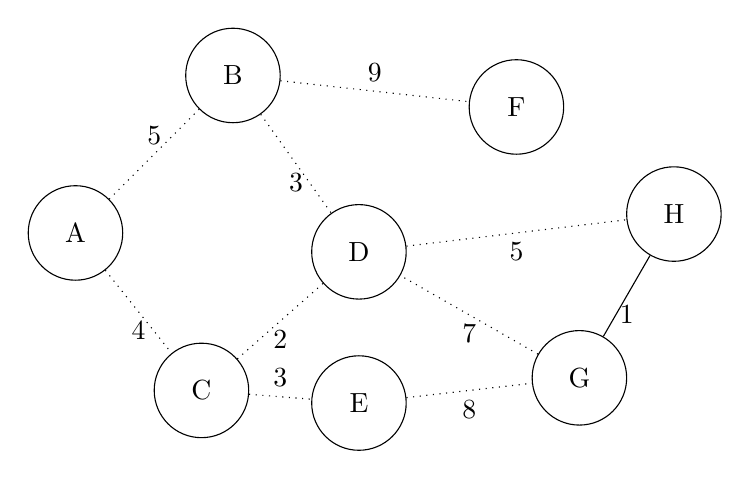
\begin{tikzpicture}[scale=0.8]
    \node[circle, draw, minimum size=1.2cm] (A) at (0, 0) {A};
    \node[circle, draw, minimum size=1.2cm] (B) at (2.5, 2.5) {B};
    \node[circle, draw, minimum size=1.2cm] (C) at (2.0, -2.5) {C};
    \node[circle, draw, minimum size=1.2cm] (D) at (4.5, -0.3) {D};
    \node[circle, draw, minimum size=1.2cm] (E) at (4.5, -2.7) {E};
    \node[circle, draw, minimum size=1.2cm] (F) at (7.0, 2.0) {F};
    \node[circle, draw, minimum size=1.2cm] (G) at (8.0, -2.3) {G};
    \node[circle, draw, minimum size=1.2cm] (H) at (9.5, 0.3) {H};

    % エッジを引く
    \draw[dotted] (A) -- node[above] {5} (B);
    \draw[dotted] (A) -- node[below] {4} (C);
    \draw[dotted] (C) -- node[above] {3} (E);
    \draw[dotted] (B) -- node[above] {9} (F);
    \draw[dotted] (E) -- node[below] {8} (G);
    \draw[dotted] (G) -- node[below] {7} (D);
    \draw[dotted] (D) -- node[below] {5} (H);
    \draw[dotted] (B) -- node[below] {3} (D);
    \draw[dotted] (C) -- node[below] {2} (D);
    \draw (G) -- node[below] {1} (H);
  \end{tikzpicture}
\end{center}

\vspace{0.5cm}

同様に、CD、CE、BD、AC、DHを順に追加しても閉路はできないので、追加します。

\vspace{0.5cm}

\begin{center}
  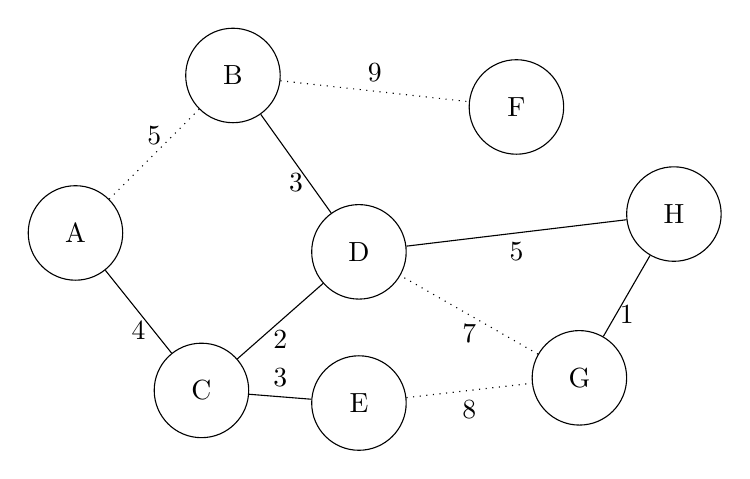
\begin{tikzpicture}[scale=0.8]
    \node[circle, draw, minimum size=1.2cm] (A) at (0, 0) {A};
    \node[circle, draw, minimum size=1.2cm] (B) at (2.5, 2.5) {B};
    \node[circle, draw, minimum size=1.2cm] (C) at (2.0, -2.5) {C};
    \node[circle, draw, minimum size=1.2cm] (D) at (4.5, -0.3) {D};
    \node[circle, draw, minimum size=1.2cm] (E) at (4.5, -2.7) {E};
    \node[circle, draw, minimum size=1.2cm] (F) at (7.0, 2.0) {F};
    \node[circle, draw, minimum size=1.2cm] (G) at (8.0, -2.3) {G};
    \node[circle, draw, minimum size=1.2cm] (H) at (9.5, 0.3) {H};

    % エッジを引く
    \draw[dotted] (A) -- node[above] {5} (B);
    \draw (A) -- node[below] {4} (C);
    \draw (C) -- node[above] {3} (E);
    \draw[dotted] (B) -- node[above] {9} (F);
    \draw[dotted] (E) -- node[below] {8} (G);
    \draw[dotted] (G) -- node[below] {7} (D);
    \draw (D) -- node[below] {5} (H);
    \draw (B) -- node[below] {3} (D);
    \draw (C) -- node[below] {2} (D);
    \draw (G) -- node[below] {1} (H);
  \end{tikzpicture}
\end{center}

\vspace{0.5cm}
しかし、AB、DG、EGを繋げると閉路ができてしまうので追加しません。最後にBFを追加するとすべての辺をチェックし終えたので以下のような
最小全域木ができあがります。

\vspace{0.5cm}

\begin{center}
  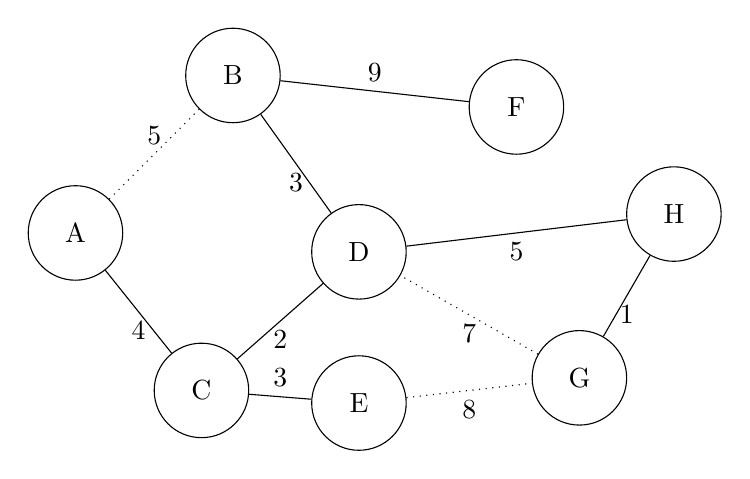
\begin{tikzpicture}[scale=0.8]
    \node[circle, draw, minimum size=1.2cm] (A) at (0, 0) {A};
    \node[circle, draw, minimum size=1.2cm] (B) at (2.5, 2.5) {B};
    \node[circle, draw, minimum size=1.2cm] (C) at (2.0, -2.5) {C};
    \node[circle, draw, minimum size=1.2cm] (D) at (4.5, -0.3) {D};
    \node[circle, draw, minimum size=1.2cm] (E) at (4.5, -2.7) {E};
    \node[circle, draw, minimum size=1.2cm] (F) at (7.0, 2.0) {F};
    \node[circle, draw, minimum size=1.2cm] (G) at (8.0, -2.3) {G};
    \node[circle, draw, minimum size=1.2cm] (H) at (9.5, 0.3) {H};

    % エッジを引く
    \draw[dotted] (A) -- node[above] {5} (B);
    \draw (A) -- node[below] {4} (C);
    \draw (C) -- node[above] {3} (E);
    \draw (B) -- node[above] {9} (F);
    \draw[dotted] (E) -- node[below] {8} (G);
    \draw[dotted] (G) -- node[below] {7} (D);
    \draw (D) -- node[below] {5} (H);
    \draw (B) -- node[below] {3} (D);
    \draw (C) -- node[below] {2} (D);
    \draw (G) -- node[below] {1} (H);
  \end{tikzpicture}
\end{center}

\vspace{0.5cm}

クラスカル法の実装上のポイントは以下の2つです。

\begin{itemize}
  \item すべての辺を重さの小さい順にソートする
  \item 辺を追加したときに閉路かどうかを判定する
\end{itemize}

最初のポイントは、辺を重さの小さい順にソートすることで、簡単に実装できます。2つ目のポイントは、BFSやDFSを使っても実装できますが、効率が良くありません。
そこで、Union-Find木を使って実装することが一般的です。

ある辺をグラフに木に挿入しようとしたとき、辺を作る2点が同じ集合に属している場合に辺を繋げると閉路が
できてしまいます。つまり、Union-Findを使ってふたつのノードが同じ集合に属しているかを判断します。

\begin{lstlisting}[caption=クラスカル法の実装, label=kruskal, frame=TRBL, label={kruskal}]
class UnionFind:
  def __init__(self, n: int) -> None:
      self.parent = [i for i in range(n)]
      self.rank = [0] * n
  
  def _root(self, node: int) -> int:
      if self.parent[node] == node:
          return node
      else:
          # 経路圧縮
          self.parent[node] = self._root(node)
          return self.parent[node]
  
  def unite(self, x: int, y: int) -> None:
      root_x = self._root(x)
      root_y = self._root(y)
      
      if root_x != root_y:
          if self.rank[root_x] < self.rank[root_y]:
              self.parent[root_x] = root_y
          else:
              self.parent[root_y] = root_x
              if self.parent[root_x] == self.parent[root_y]:
                  self.rank[root_x] += 1
  def is_same(self, x: int, y: int) -> bool:
      return self.parent[x] == self.parent[y]

def kruskal(v: int, edges: list[tuple[int, int, int]]) -> list[list[int, int]]:
    """
    args:
        v: node size
        edges: (start, end, weight)
    """
    sorted_edge_costs = []
    for edge in edges:
        sorted_edge_costs.append([edges[2], edges[0], edges[1]])
    
    sorted_edge_costs.sort()
    
    uf_tree = UnionFind(v)
    
    minimum_spanning_tree = []
    
    for weight, start, end in sorted_edge_costs:
        if not uf_tree.is_same(start, end):
            uf_tree.unite(start, end)
            minimum_spanning_tree.append([start, end])
    
    return minimum_spanning_tree
\end{lstlisting}

\newpage

\subsection{プリム法}
\textbf{プリム法}とは、すでに到達した頂点の集合からまだ到達していない頂点の集合への辺のうち、距離が
最短のものを追加し、すべてのノードがつながったら終了するアルゴリズムです。プリム法は以下のアルゴリズム
に従っています。

\begin{enumerate}
  \item 任意のノードを選び、訪問済みにする
  \item そのノードに繋がっているすべての辺を最小全域木の候補の辺として追加する
  \item 最小全域木の候補の辺の中から、接続先のノードが未訪問である最短の距離の辺を選ぶ
  \item 選んだ辺を最小全域木に入れ、その接続先のノードを訪問済にする。 
  \item 4で新しく訪問したノードから、さらにその先に繋がっている辺のうち、接続先のノードが未訪問のすべての辺を最小全域木の候補に追加する
  \item すべてのノードが訪問済になるまで2から4を繰り返す
\end{enumerate}

プリム法の具体例を見てみましょう。まずは、任意にノードを選び、訪問済にします。ここではDを選びます。Dから繋がっているエッジを青色で示します。その中で
最も距離が短いエッジはCとDを繋ぐエッジです。

\vspace{0.5cm}

\begin{center}
  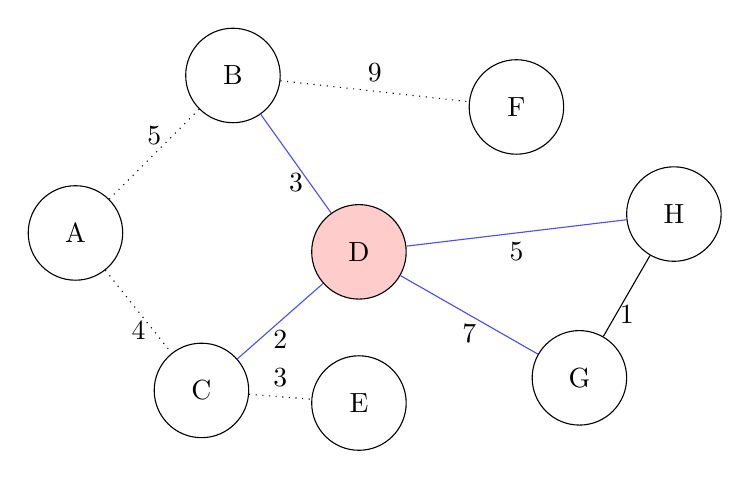
\begin{tikzpicture}[scale=0.8]
    \node[circle, draw, minimum size=1.2cm] (A) at (0, 0) {A};
    \node[circle, draw, minimum size=1.2cm] (B) at (2.5, 2.5) {B};
    \node[circle, draw, minimum size=1.2cm] (C) at (2.0, -2.5) {C};
    \node[circle, draw, minimum size=1.2cm, fill=red!20] (D) at (4.5, -0.3) {D};
    \node[circle, draw, minimum size=1.2cm] (E) at (4.5, -2.7) {E};
    \node[circle, draw, minimum size=1.2cm] (F) at (7.0, 2.0) {F};
    \node[circle, draw, minimum size=1.2cm] (G) at (8.0, -2.3) {G};
    \node[circle, draw, minimum size=1.2cm] (H) at (9.5, 0.3) {H};

    % エッジを引く
    \draw[dotted] (A) -- node[above] {5} (B);
    \draw[dotted] (A) -- node[below] {4} (C);
    \draw[dotted] (C) -- node[above] {3} (E);
    \draw[dotted] (B) -- node[above] {9} (F);
    \draw[draw=blue!70] (G) -- node[below] {7} (D);
    \draw[draw=blue!70] (D) -- node[below] {5} (H);
    \draw[draw=blue!70] (B) -- node[below] {3} (D);
    \draw[draw=blue!70] (C) -- node[below] {2} (D);
    \draw[] (G) -- node[below] {1} (H);
  \end{tikzpicture}
\end{center}

Cは未訪問なので、Cを訪問済にして、Cから繋がっているエッジを最小全域木の候補に追加します。青色のエッジの中で
距離が一番小さいエッジはBとDを繋ぐエッジです。

\begin{center}
  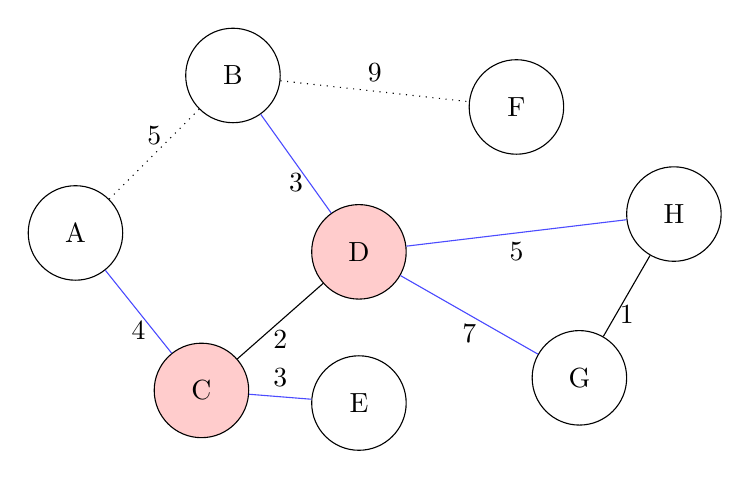
\begin{tikzpicture}[scale=0.8]
    \node[circle, draw, minimum size=1.2cm] (A) at (0, 0) {A};
    \node[circle, draw, minimum size=1.2cm] (B) at (2.5, 2.5) {B};
    \node[circle, draw, minimum size=1.2cm, fill=red!20] (C) at (2.0, -2.5) {C};
    \node[circle, draw, minimum size=1.2cm, fill=red!20] (D) at (4.5, -0.3) {D};
    \node[circle, draw, minimum size=1.2cm] (E) at (4.5, -2.7) {E};
    \node[circle, draw, minimum size=1.2cm] (F) at (7.0, 2.0) {F};
    \node[circle, draw, minimum size=1.2cm] (G) at (8.0, -2.3) {G};
    \node[circle, draw, minimum size=1.2cm] (H) at (9.5, 0.3) {H};

    % エッジを引く
    \draw[dotted] (A) -- node[above] {5} (B);
    \draw[draw=blue!70] (A) -- node[below] {4} (C);
    \draw[draw=blue!70] (C) -- node[above] {3} (E);
    \draw[dotted] (B) -- node[above] {9} (F);
    \draw[draw=blue!70] (G) -- node[below] {7} (D);
    \draw[draw=blue!70] (D) -- node[below] {5} (H);
    \draw[draw=blue!70] (B) -- node[below] {3} (D);
    \draw (C) -- node[below] {2} (D);
    \draw[] (G) -- node[below] {1} (H);
  \end{tikzpicture}
\end{center}

Bは未訪問なので、Bを訪問済にして、Bから繋がっているエッジを最小全域木の候補に追加します。青色のエッジの中で
最も短いエッジはCとEを繋ぐエッジです。

\vspace{0.5cm}

\begin{center}
  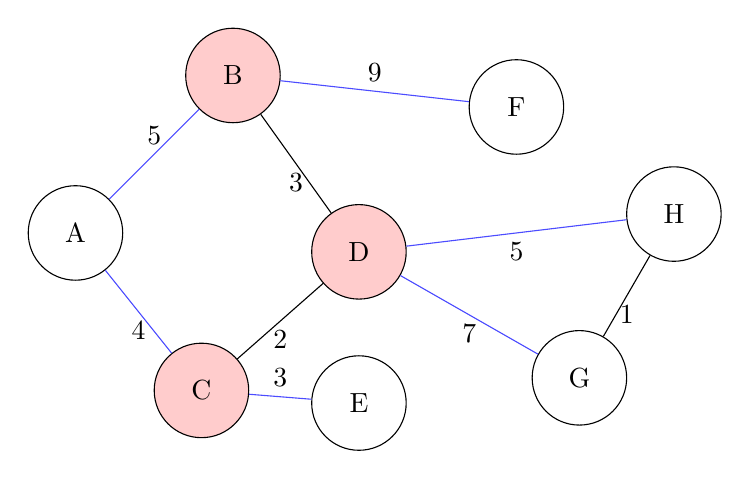
\begin{tikzpicture}[scale=0.8]
    \node[circle, draw, minimum size=1.2cm] (A) at (0, 0) {A};
    \node[circle, draw, minimum size=1.2cm, fill=red!20] (B) at (2.5, 2.5) {B};
    \node[circle, draw, minimum size=1.2cm, fill=red!20] (C) at (2.0, -2.5) {C};
    \node[circle, draw, minimum size=1.2cm, fill=red!20] (D) at (4.5, -0.3) {D};
    \node[circle, draw, minimum size=1.2cm] (E) at (4.5, -2.7) {E};
    \node[circle, draw, minimum size=1.2cm] (F) at (7.0, 2.0) {F};
    \node[circle, draw, minimum size=1.2cm] (G) at (8.0, -2.3) {G};
    \node[circle, draw, minimum size=1.2cm] (H) at (9.5, 0.3) {H};

    % エッジを引く
    \draw[draw=blue!70] (A) -- node[above] {5} (B);
    \draw[draw=blue!70] (A) -- node[below] {4} (C);
    \draw[draw=blue!70] (C) -- node[above] {3} (E);
    \draw[draw=blue!70] (B) -- node[above] {9} (F);
    \draw[draw=blue!70] (G) -- node[below] {7} (D);
    \draw[draw=blue!70] (D) -- node[below] {5} (H);
    \draw (B) -- node[below] {3} (D);
    \draw (C) -- node[below] {2} (D);
    \draw[] (G) -- node[below] {1} (H);
  \end{tikzpicture}
\end{center}

同様にして、AとCを結ぶエッジ、DとHを結ぶエッジ、GとHを結ぶエッジを追加します。

\vspace{0.5cm}

\begin{center}
  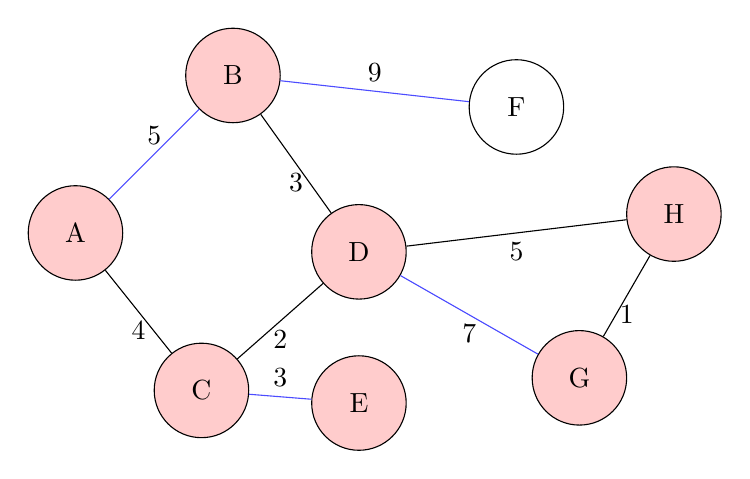
\begin{tikzpicture}[scale=0.8]
    \node[circle, draw, minimum size=1.2cm, fill=red!20] (A) at (0, 0) {A};
    \node[circle, draw, minimum size=1.2cm, fill=red!20] (B) at (2.5, 2.5) {B};
    \node[circle, draw, minimum size=1.2cm, fill=red!20] (C) at (2.0, -2.5) {C};
    \node[circle, draw, minimum size=1.2cm, fill=red!20] (D) at (4.5, -0.3) {D};
    \node[circle, draw, minimum size=1.2cm, fill=red!20] (E) at (4.5, -2.7) {E};
    \node[circle, draw, minimum size=1.2cm] (F) at (7.0, 2.0) {F};
    \node[circle, draw, minimum size=1.2cm, fill=red!20] (G) at (8.0, -2.3) {G};
    \node[circle, draw, minimum size=1.2cm, fill=red!20] (H) at (9.5, 0.3) {H};

    % エッジを引く
    \draw[draw=blue!70] (A) -- node[above] {5} (B);
    \draw (A) -- node[below] {4} (C);
    \draw[draw=blue!70] (C) -- node[above] {3} (E);
    \draw[draw=blue!70] (B) -- node[above] {9} (F);
    \draw[draw=blue!70] (G) -- node[below] {7} (D);
    \draw (D) -- node[below] {5} (H);
    \draw (B) -- node[below] {3} (D);
    \draw (C) -- node[below] {2} (D);
    \draw[] (G) -- node[below] {1} (H);
  \end{tikzpicture}
\end{center}

\vspace{0.5cm}

残りは、AとBを結ぶエッジ、DとGを結ぶエッジがありますが、AとBを結ぶエッジとDとGを結ぶエッジを追加すると閉路ができてしまうので追加しません。
最後にDとGを結ぶエッジを追加すると、すべてのノードがつながったので終了です。以下のような最小全域木ができあがります。

\vspace{0.5cm}

\begin{center}
  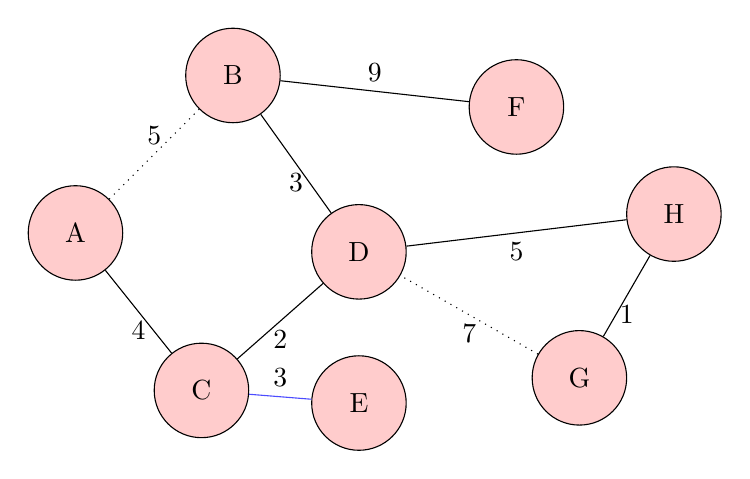
\begin{tikzpicture}[scale=0.8]
    \node[circle, draw, minimum size=1.2cm, fill=red!20] (A) at (0, 0) {A};
    \node[circle, draw, minimum size=1.2cm, fill=red!20] (B) at (2.5, 2.5) {B};
    \node[circle, draw, minimum size=1.2cm, fill=red!20] (C) at (2.0, -2.5) {C};
    \node[circle, draw, minimum size=1.2cm, fill=red!20] (D) at (4.5, -0.3) {D};
    \node[circle, draw, minimum size=1.2cm, fill=red!20] (E) at (4.5, -2.7) {E};
    \node[circle, draw, minimum size=1.2cm,fill=red!20] (F) at (7.0, 2.0) {F};
    \node[circle, draw, minimum size=1.2cm, fill=red!20] (G) at (8.0, -2.3) {G};
    \node[circle, draw, minimum size=1.2cm, fill=red!20] (H) at (9.5, 0.3) {H};

    % エッジを引く
    \draw[dotted] (A) -- node[above] {5} (B);
    \draw (A) -- node[below] {4} (C);
    \draw[draw=blue!70] (C) -- node[above] {3} (E);
    \draw (B) -- node[above] {9} (F);
    \draw[dotted] (G) -- node[below] {7} (D);
    \draw (D) -- node[below] {5} (H);
    \draw (B) -- node[below] {3} (D);
    \draw (C) -- node[below] {2} (D);
    \draw[] (G) -- node[below] {1} (H);
  \end{tikzpicture}
\end{center}

\vspace{0.5cm}

プリム法の実装例を以下に示します。

\begin{lstlisting}[caption=プリム法の実装, label=prim, frame=TRBL, label={prim}]
import heapq

def prim(v: int, edges: list[list[int, int, int]]):
    edges_from = [[] for _ in range(v)]
    
    for start, end, weight in edges:
        edges_from[start].append([weight, start, end])
    
    edge_heap = []
    minimum_spanning_tree = []
    included = [False] * v
    
    # nodeをひとつ選ぶ この実装では0を選ぶ
    included[0] = True
    # node0につながる辺をすべてヒープに入れる
    for edge in edges_from[0]:
        heapq.heappush(edge_heap, edge)
    
    while edge_heap:
        weight, start, end = heapq.heappop(edge_heap)
        if not included[end]:
            included[end] = True
            minimum_spanning_tree.append([start, end])
            
            for edge in edges_from[end]:
                if not included[end]:
                    heapq.heappush(edge_heap, edge)
    
    return minimum_spanning_tree
\end{lstlisting}

\newpage

\section{トポロジカルソート}
DAGという性質を持ったグラフをソートするアルゴリズムであるトポロジカルソートを扱います。\textbf{DAG}(Directed Acyclic Graph)
とは、その名の通り有向グラフで閉路を持たないグラフのことを指します。

以下にDAGの例を示します。有向グラフで閉路がないため、どこのノードから辿っても元の位置に戻ってくることはできません。

\begin{center}
  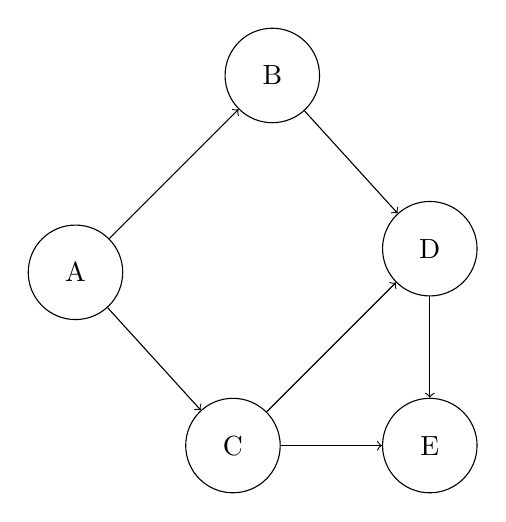
\begin{tikzpicture}
    \node[circle, draw, minimum size=1.2cm] (A) at (0, 0) {A};
    \node[circle, draw, minimum size=1.2cm] (B) at (2.5, 2.5) {B};
    \node[circle, draw, minimum size=1.2cm] (C) at (2.0, -2.2) {C};
    \node[circle, draw, minimum size=1.2cm] (D) at (4.5, 0.3) {D};
    \node[circle, draw, minimum size=1.2cm] (E) at (4.5, -2.2) {E};

    \draw[->] (A) -- (B);
    \draw[->] (A) -- (C);
    \draw[->] (B) -- (D);
    \draw[->] (C) -- (D);
    \draw[->] (C) -- (E);
    \draw[->] (D) -- (E);
  \end{tikzpicture}
\end{center}

\begin{center}
  DAGの例
\end{center}

\vspace{0.5cm}

トポロジカルソートはすべての辺が同じ方向を向くようにノードをソートするアルゴリズムです。上のDAGをトポロジカルソートをすると、
以下のようになります。有向辺がすべて右向きになっていることがわかります。注意点として、トポロジカルソートの結果は
一意ではありません。

\vspace{0.5cm}

\begin{center}
  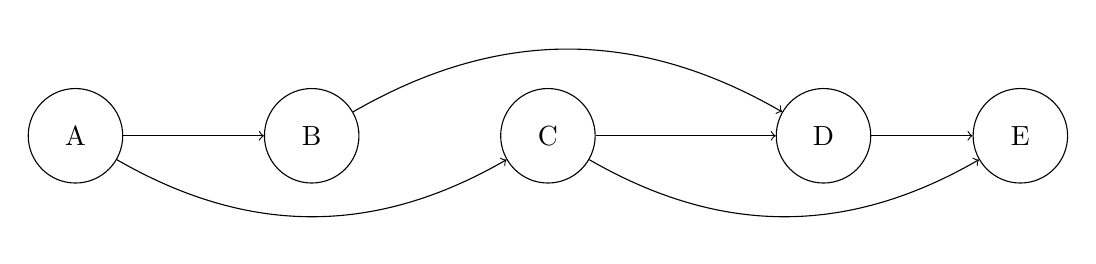
\begin{tikzpicture}
    \node[circle, draw, minimum size=1.2cm] (A) at (0, 0) {A};
    \node[circle, draw, minimum size=1.2cm] (B) at (3, 0) {B};
    \node[circle, draw, minimum size=1.2cm] (C) at (6.0, 0) {C};
    \node[circle, draw, minimum size=1.2cm] (D) at (9.5, 0) {D};
    \node[circle, draw, minimum size=1.2cm] (E) at (12, -0) {E};

    \draw[->] (A) to (B);
    \draw[->, bend right] (A) to (C);
    \draw[->, bend left] (B) to (D);
    \draw[->] (C) to (D);
    \draw[->, bend right] (C) to (E);
    \draw[->] (D) to (E);
  \end{tikzpicture}
\end{center}

\vspace{0.5cm}

有向グラフの性質をより理解するために\textbf{次数、入次数、出次数}という用語を導入します。次数とは、ノードにつながっている辺の数を指します。
入次数とは、ノードに入ってくる辺の数を指し、出次数とは、ノードから出ていく辺の数を指します。$\text{次数} = \text{入次数} + \text{出次数}$です。
DAGの性質として、必ず入次数0のノードが存在します。

トポロジカルソートの代表的なアルゴリズムとして、KahnのアルゴリズムとTarjanのアルゴリズムを紹介します。

\subsection{Kahnのアルゴリズム}
Kahnのアルゴリズムは、トポロジカルソートを行うアルゴリズムの一つです。アルゴリズムの流れは以下の通りです。

\begin{enumerate}
  \item 入次数が0のノードをグラフから取り除き、ソート済配列に追加する
  \item 1を入次数0のノードがなくなるまで繰り返す
\end{enumerate}

Kahnのアルゴリズムの例を以下に示します。

\vspace{0.5cm}

\begin{center}
  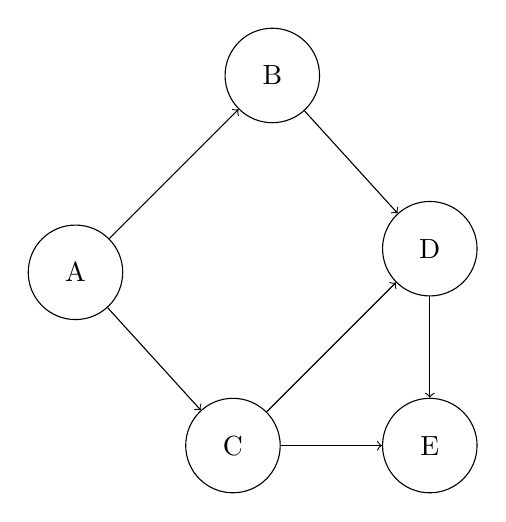
\begin{tikzpicture}
    \node[circle, draw, minimum size=1.2cm] (A) at (0, 0) {A};
    \node[circle, draw, minimum size=1.2cm] (B) at (2.5, 2.5) {B};
    \node[circle, draw, minimum size=1.2cm] (C) at (2.0, -2.2) {C};
    \node[circle, draw, minimum size=1.2cm] (D) at (4.5, 0.3) {D};
    \node[circle, draw, minimum size=1.2cm] (E) at (4.5, -2.2) {E};

    \draw[->] (A) -- (B);
    \draw[->] (A) -- (C);
    \draw[->] (B) -- (D);
    \draw[->] (C) -- (D);
    \draw[->] (C) -- (E);
    \draw[->] (D) -- (E);
  \end{tikzpicture}
\end{center}

\vspace{0.5cm}

入次数0のノードAを取り除き、Aに繋がっているノードの次数を更新します。

\vspace{0.5cm}

\begin{center}
  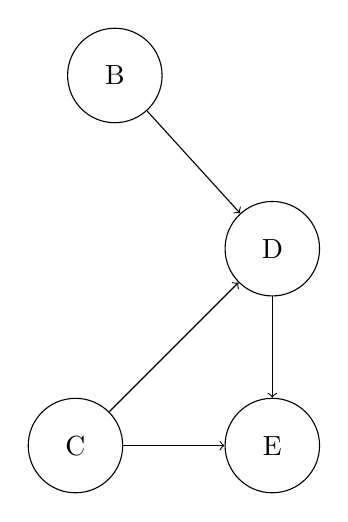
\begin{tikzpicture}
    \node[circle, draw, minimum size=1.2cm] (B) at (2.5, 2.5) {B};
    \node[circle, draw, minimum size=1.2cm] (C) at (2.0, -2.2) {C};
    \node[circle, draw, minimum size=1.2cm] (D) at (4.5, 0.3) {D};
    \node[circle, draw, minimum size=1.2cm] (E) at (4.5, -2.2) {E};

    \draw[->] (B) -- (D);
    \draw[->] (C) -- (D);
    \draw[->] (C) -- (E);
    \draw[->] (D) -- (E);
  \end{tikzpicture}
\end{center}

\vspace{0.5cm}

入次数0のノードBを取り除きます。


\vspace{0.5cm}

\begin{center}
  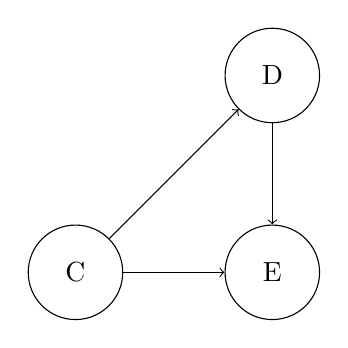
\begin{tikzpicture}
    \node[circle, draw, minimum size=1.2cm] (C) at (2.0, -2.2) {C};
    \node[circle, draw, minimum size=1.2cm] (D) at (4.5, 0.3) {D};
    \node[circle, draw, minimum size=1.2cm] (E) at (4.5, -2.2) {E};

    \draw[->] (C) -- (D);
    \draw[->] (C) -- (E);
    \draw[->] (D) -- (E);
  \end{tikzpicture}
\end{center}

\vspace{0.5cm}

入次数0のノードCを取り除きます。最後にノードDとEを順に取り出せばトポロジカルソートは完成です。


\vspace{0.5cm}

\begin{center}
  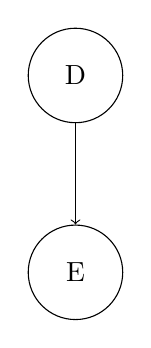
\begin{tikzpicture}
    \node[circle, draw, minimum size=1.2cm] (D) at (4.5, 0.3) {D};
    \node[circle, draw, minimum size=1.2cm] (E) at (4.5, -2.2) {E};

    \draw[->] (D) -- (E);
  \end{tikzpicture}
\end{center}

\vspace{0.5cm}

Kahnのアルゴリズムの実装例を以下に示します。
\begin{lstlisting}[caption=Kahnのアルゴリズムの実装, label=kahn, frame=TRBL, label={kahn}]
from collections import deque

def kahn_topological_sort(v: int, e: int, edges: list[list[int, int]]) -> list[int]:
    indeg = [0] * v
    outedge = [[] for _ in range(v)]
    
    for start, end in edges:
        indeg[end] += 1
        outedge[start].append[end]
    
    sorted_g = [i for i in range(v) if indeg[i] == 0]
    deq = deque(sorted_g)
    
    while deq:
        node = deq.popleft()
        for connected_node in outedge[node]:
            e -= 1
            indeg[connected_node] -= 1
            if indeg[connected_node] == 0: 
                sorted_g.append(connected_node)
                deq.append(connected_node)
    
    if e != 0:
        return None
    
    return sorted_g
\end{lstlisting}

\subsection{Tarjanのアルゴリズム}
Tarjanのアルゴリズムは、深さ優先探索を用いてトポロジカルソートを行うアルゴリズムです。アルゴリズムの流れは以下の通りです。

\begin{enumerate}
  \item 未訪問のノードを訪問済にする
  \item そのノードに繋がっているノードを再帰的に訪問する
  \item そのノードのすべての子ノードを訪問し終えたら、そのノードをソート済配列に追加する
\end{enumerate}

Tarjanのアルゴリズムの実装例を以下に示します。

\begin{lstlisting}[caption=Tarjanのアルゴリズムの実装, label=tarjan, frame=TRBL, label={tarjan}]
def tarjan_topological_sort(v: int, edges: list[list[int, int]]) -> list[int]:
    def dfs(node: int):
        visited[node] = True
        for connected_node in outedge[node]:
            if not visited[connected_node]:
                dfs(connected_node)
        sorted_g.append(node)
    
    outedge = [[] for _ in range(v)]
    visited = [False] * v
    sorted_g = []
    
    for start, end in edges:
        outedge[start].append(end)
    
    for i in range(v):
        if not visited[i]:
            dfs(i)
    
    return sorted_g[::-1]
\end{lstlisting}

\newpage

\section{最大流問題}
グラフに流れ(フロー)があるグラフを考えます。特に、フローは始点(source)のみから生まれ、終点(sink)でのみ消滅するという性質を持つ場合を考えます。
グラフでフローを扱う分野をネットワークフローといいます。エッジに容量を導入して、各エッジを通るフローの量が容量を超えないという条件のもとで終点に最も多くのフローを流す問題を\textbf{最大流問題}といいます。

\vspace{0.5cm}

\begin{center}
  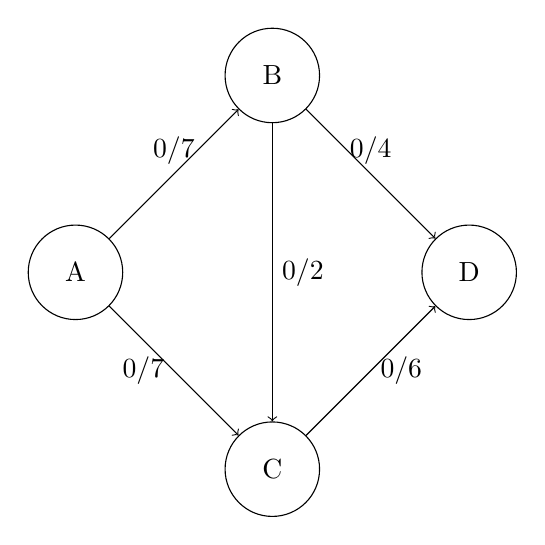
\begin{tikzpicture}
    \node[circle, draw, minimum size=1.2cm] (A) at (0, 0) {A};
    \node[circle, draw, minimum size=1.2cm] (B) at (2.5, 2.5) {B};
    \node[circle, draw, minimum size=1.2cm] (C) at (2.5, -2.5) {C};
    \node[circle, draw, minimum size=1.2cm] (D) at (5, 0) {D};

    \draw[->] (A) -- node[above] {0/7} (B);
    \draw[->] (A) -- node[left] {0/7} (C);
    \draw[->] (B) -- node[above] {0/4} (D);
    \draw[->] (C) -- node[right] {0/6} (D);
    \draw[->] (B) -- node[right] {0/2} (C);
  \end{tikzpicture}
\end{center}

\vspace{0.5cm}

\subsection{最大流問題と貪欲法の限界}
DFSを使って見つかった道から順番にフローを流す貪欲法から考えてみます。下のネットワークグラフを例にして考えます。Aをsource、Fをsinkとして例を挙げます。

\vspace{0.5cm}

\begin{center}
  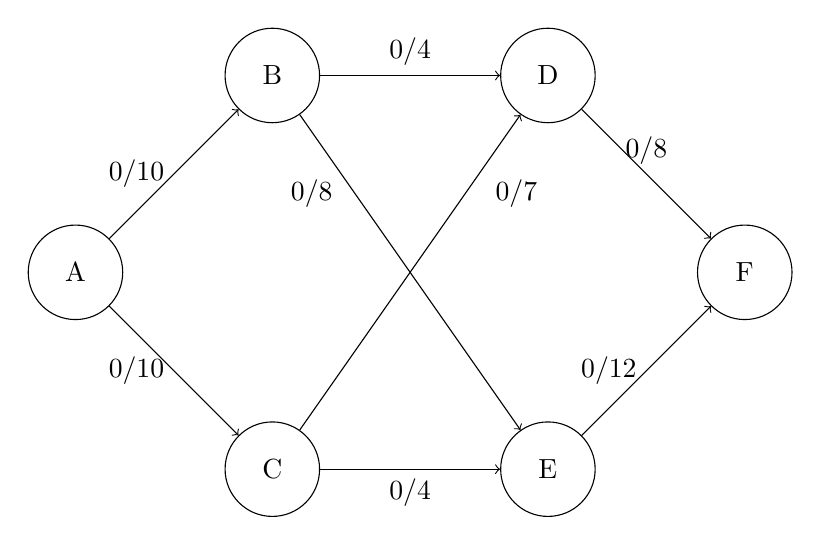
\begin{tikzpicture}
    \node[circle, draw, minimum size=1.2cm] (A) at (0, 0) {A};
    \node[circle, draw, minimum size=1.2cm] (B) at (2.5, 2.5) {B};
    \node[circle, draw, minimum size=1.2cm] (C) at (2.5, -2.5) {C};
    \node[circle, draw, minimum size=1.2cm] (D) at (6, 2.5) {D};
    \node[circle, draw, minimum size=1.2cm] (E) at (6, -2.5) {E};
    \node[circle, draw, minimum size=1.2cm] (F) at (8.5, 0) {F};

    % エッジを引く
    \draw[->] (A) -- node[left] {0/10} (B);
    \draw[->] (A) -- node[left] {0/10} (C);
    \draw[->] (B) -- node[above] {0/4} (D);
    \draw[->] (B) -- (E);
    \draw[->] (C) -- node[below] {0/4} (E);
    \draw[->] (E) -- node[left] {0/12} (F);
    \draw[->] (D) -- node[above] {0/8} (F);
    \draw[->] (C) -- (D);

    % 容量を書く
    \node at (3, 1) {0/8};
    \node at (5.6, 1) {0/7};

    % 赤い太線で線を引く
    % \draw[draw=red, very thick, ->] (A) -- (B);
  \end{tikzpicture}
\end{center}

\vspace{0.5cm}

  DFSを使って順番に経路を見つけていきます。最初はABDFの経路にフローを流してみます。この経路の中で容量が最も小さい
  経路に合わせて流さないと溢れてしまうので、今回はBDの経路の容量の4を流します。

\vspace{0.5cm}

\begin{center}
  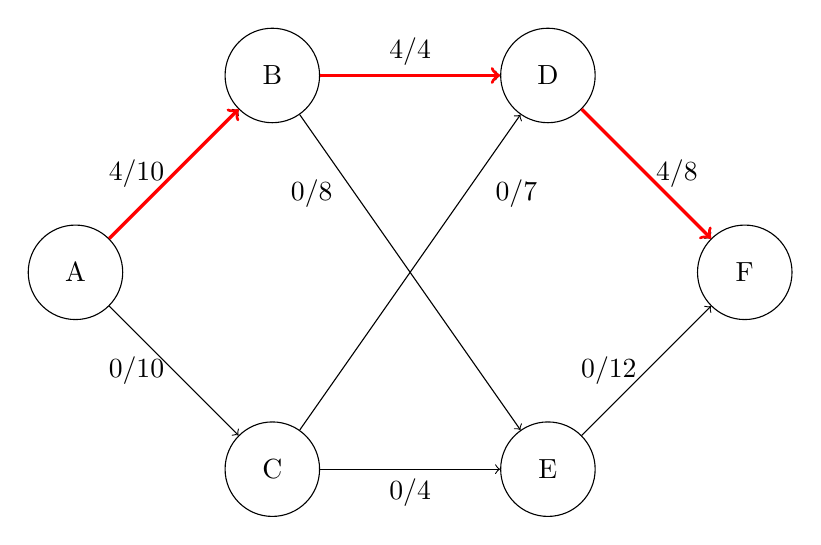
\begin{tikzpicture}
    \node[circle, draw, minimum size=1.2cm] (A) at (0, 0) {A};
    \node[circle, draw, minimum size=1.2cm] (B) at (2.5, 2.5) {B};
    \node[circle, draw, minimum size=1.2cm] (C) at (2.5, -2.5) {C};
    \node[circle, draw, minimum size=1.2cm] (D) at (6, 2.5) {D};
    \node[circle, draw, minimum size=1.2cm] (E) at (6, -2.5) {E};
    \node[circle, draw, minimum size=1.2cm] (F) at (8.5, 0) {F};

    % エッジを引く
    \draw[->] (A) -- node[left] {4/10} (B);
    \draw[->] (A) -- node[left] {0/10} (C);
    \draw[->] (B) -- node[above] {4/4} (D);
    \draw[->] (B) -- (E);
    \draw[->] (C) -- node[below] {0/4} (E);
    \draw[->] (E) -- node[left] {0/12} (F);
    \draw[->] (D) -- node[right] {4/8} (F);
    \draw[->] (C) -- (D);

    % 容量を書く
    \node at (3, 1) {0/8};
    \node at (5.6, 1) {0/7};

    % 赤い太線で線を引く
    \draw[draw=red, very thick, ->] (A) -- (B);
    \draw[draw=red, very thick, ->] (B) -- (D);
    \draw[draw=red, very thick, ->] (D) -- (F);
  \end{tikzpicture} 
\end{center}

\vspace{0.5cm}

次にABEFの経路にフローを流します。経路を見ているとABの経路は残り6のフローを流せてABEFの経路で最も小さい経路なので、
6のフローを流します。


\vspace{0.5cm}

\begin{center}
  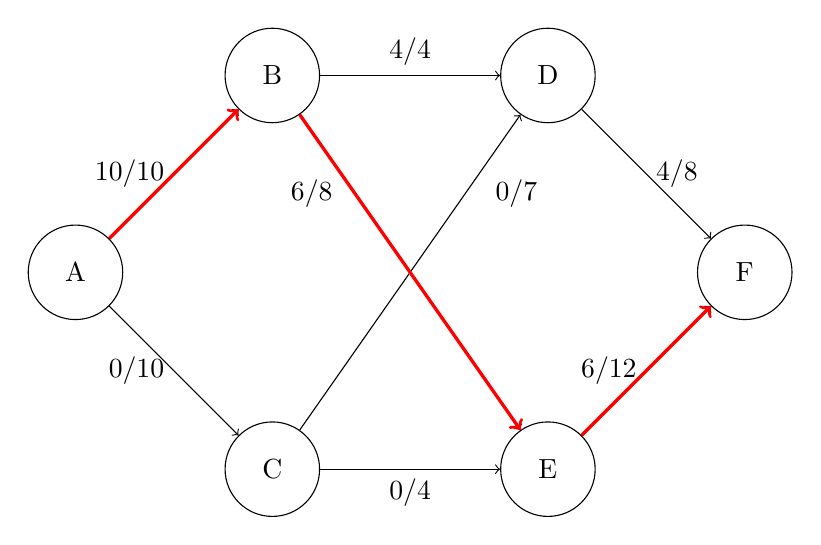
\begin{tikzpicture}
    \node[circle, draw, minimum size=1.2cm] (A) at (0, 0) {A};
    \node[circle, draw, minimum size=1.2cm] (B) at (2.5, 2.5) {B};
    \node[circle, draw, minimum size=1.2cm] (C) at (2.5, -2.5) {C};
    \node[circle, draw, minimum size=1.2cm] (D) at (6, 2.5) {D};
    \node[circle, draw, minimum size=1.2cm] (E) at (6, -2.5) {E};
    \node[circle, draw, minimum size=1.2cm] (F) at (8.5, 0) {F};

    % エッジを引く
    \draw[->] (A) -- node[left] {10/10} (B);
    \draw[->] (A) -- node[left] {0/10} (C);
    \draw[->] (B) -- node[above] {4/4} (D);
    \draw[->] (B) -- (E);
    \draw[->] (C) -- node[below] {0/4} (E);
    \draw[->] (E) -- node[left] {6/12} (F);
    \draw[->] (D) -- node[right] {4/8} (F);
    \draw[->] (C) -- (D);

    % 容量を書く
    \node at (3, 1) {6/8};
    \node at (5.6, 1) {0/7};

    % 赤い太線で線を引く
    \draw[draw=red, very thick, ->] (A) -- (B);
    \draw[draw=red, very thick, ->] (B) -- (E);
    \draw[draw=red, very thick, ->] (E) -- (F);
  \end{tikzpicture} 
\end{center}

\vspace{0.5cm}

次にACDFの経路を考える。DFの残り容量4が経路の中で最も小さな容量なので、4のフローを流します。

\vspace{0.5cm}

\begin{center}
  \begin{tikzpicture}
    \node[circle, draw, minimum size=1.2cm] (A) at (0, 0) {A};
    \node[circle, draw, minimum size=1.2cm] (B) at (2.5, 2.5) {B};
    \node[circle, draw, minimum size=1.2cm] (C) at (2.5, -2.5) {C};
    \node[circle, draw, minimum size=1.2cm] (D) at (6, 2.5) {D};
    \node[circle, draw, minimum size=1.2cm] (E) at (6, -2.5) {E};
    \node[circle, draw, minimum size=1.2cm] (F) at (8.5, 0) {F};

    % エッジを引く
    \draw[->] (A) -- node[left] {10/10} (B);
    \draw[->] (A) -- node[left] {4/10} (C);
    \draw[->] (B) -- node[above] {4/4} (D);
    \draw[->] (B) -- (E);
    \draw[->] (C) -- node[below] {0/4} (E);
    \draw[->] (E) -- node[left] {6/12} (F);
    \draw[->] (D) -- node[right] {8/8} (F);
    \draw[->] (C) -- (D);

    % 容量を書く
    \node at (3, 1) {6/8};
    \node at (5.6, 1) {4/7};

    % 赤い太線で線を引く
    \draw[draw=red, very thick, ->] (A) -- (C);
    \draw[draw=red, very thick, ->] (C) -- (D);
    \draw[draw=red, very thick, ->] (D) -- (F);
  \end{tikzpicture} 
\end{center}

\vspace{0.5cm}

次はACEFの経路を考える。経路CEの残り容量4が経路の中で最小の容量になっているので、フロー4を流します。

\vspace{0.5cm}

\begin{center}
  \begin{tikzpicture}
    \node[circle, draw, minimum size=1.2cm] (A) at (0, 0) {A};
    \node[circle, draw, minimum size=1.2cm] (B) at (2.5, 2.5) {B};
    \node[circle, draw, minimum size=1.2cm] (C) at (2.5, -2.5) {C};
    \node[circle, draw, minimum size=1.2cm] (D) at (6, 2.5) {D};
    \node[circle, draw, minimum size=1.2cm] (E) at (6, -2.5) {E};
    \node[circle, draw, minimum size=1.2cm] (F) at (8.5, 0) {F};

    % エッジを引く
    \draw[->] (A) -- node[left] {10/10} (B);
    \draw[->] (A) -- node[left] {8/10} (C);
    \draw[->] (B) -- node[above] {4/4} (D);
    \draw[->] (B) -- (E);
    \draw[->] (C) -- node[below] {4/4} (E);
    \draw[->] (E) -- node[left] {10/12} (F);
    \draw[->] (D) -- node[right] {8/8} (F);
    \draw[->] (C) -- (D);

    % 容量を書く
    \node at (3, 1) {6/8};
    \node at (5.6, 1) {4/7};

    % 赤い太線で線を引く
    \draw[draw=red, very thick, ->] (A) -- (C);
    \draw[draw=red, very thick, ->] (C) -- (E);
    \draw[draw=red, very thick, ->] (E) -- (F);
  \end{tikzpicture} 
\end{center}

\vspace{0.5cm}

Fにつながっているエッジのフローを見てみると、18のフローが流れていることがわかります。しかし、このグラフの最大フローは
20です。貪欲法では最大フローを求めることができません。貪欲法によるフロート最大フローのネットワークを見比べましょう。

\vspace{0.5cm}

\begin{center}
  \begin{tabular}{ccc} 
    \begin{tikzpicture}[scale=0.8]
      \node[circle, draw, minimum size=1.2cm] (A) at (0, 0) {A};
      \node[circle, draw, minimum size=1.2cm] (B) at (2.5, 2.5) {B};
      \node[circle, draw, minimum size=1.2cm] (C) at (2.5, -2.5) {C};
      \node[circle, draw, minimum size=1.2cm] (D) at (6, 2.5) {D};
      \node[circle, draw, minimum size=1.2cm] (E) at (6, -2.5) {E};
      \node[circle, draw, minimum size=1.2cm] (F) at (8.5, 0) {F};
  
      % エッジを引く
      \draw[->] (A) -- node[left] {10/10} (B);
      \draw[->] (A) -- node[left] {8/10} (C);
      \draw[->] (B) -- node[above] {4/4} (D);
      \draw[->] (B) -- (E);
      \draw[->] (C) -- node[below] {4/4} (E);
      \draw[->] (E) -- node[left] {10/12} (F);
      \draw[->] (D) -- node[right] {8/8} (F);
      \draw[->] (C) -- (D);
  
      % 容量を書く
      \node at (3, 1) {6/8};
      \node at (5.6, 1) {4/7};
  
      % 赤い太線で線を引く
      \draw[draw=red, very thick, ->] (A) -- (C);
      \draw[draw=red, very thick, ->] (C) -- (E);
      \draw[draw=red, very thick, ->] (E) -- (F);
    \end{tikzpicture} 
    &
    \begin{tikzpicture}[scale=0.8]
      \node[circle, draw, minimum size=1.2cm] (A) at (0, 0) {A};
      \node[circle, draw, minimum size=1.2cm] (B) at (2.5, 2.5) {B};
      \node[circle, draw, minimum size=1.2cm] (C) at (2.5, -2.5) {C};
      \node[circle, draw, minimum size=1.2cm] (D) at (6, 2.5) {D};
      \node[circle, draw, minimum size=1.2cm] (E) at (6, -2.5) {E};
      \node[circle, draw, minimum size=1.2cm] (F) at (8.5, 0) {F};
  
      % エッジを引く
      \draw[->] (A) -- node[left] {10/10} (B);
      \draw[->] (A) -- node[left] {10/10} (C);
      \draw[->] (B) -- node[above] {2/4} (D);
      \draw[->] (B) -- (E);
      \draw[->] (C) -- node[below] {4/4} (E);
      \draw[->] (E) -- node[left] {12/12} (F);
      \draw[->] (D) -- node[right] {8/8} (F);
      \draw[->] (C) -- (D);
  
      % 容量を書く
      \node at (3, 1) {8/8};
      \node at (5.6, 1) {6/7};
  
      % 赤い太線で線を引く
      \draw[draw=red, very thick, ->] (A) -- (C);
      \draw[draw=red, very thick, ->] (C) -- (D);
      \draw[draw=red, very thick, ->] (D) -- (F);
    \end{tikzpicture}
  \end{tabular}
\end{center}

\hspace{2.5cm} 貪欲法によるフロー \hspace{5.5cm} 最大フロー

\vspace{0.5cm}

最大フローのネットワークから貪欲法のネットワークを引いてみましょう。
\vspace{0.5cm}

\begin{center}
  \begin{tikzpicture}
    \node[circle, draw, minimum size=1.2cm] (A) at (0, 0) {A};
    \node[circle, draw, minimum size=1.2cm] (B) at (2.5, 2.5) {B};
    \node[circle, draw, minimum size=1.2cm] (C) at (2.5, -2.5) {C};
    \node[circle, draw, minimum size=1.2cm] (D) at (6, 2.5) {D};
    \node[circle, draw, minimum size=1.2cm] (E) at (6, -2.5) {E};
    \node[circle, draw, minimum size=1.2cm] (F) at (8.5, 0) {F};

    % エッジを引く
    \draw[->] (A) -- node[left] {2/10} (B);
    \draw[->] (A) -- node[left] {8/10} (C);
    \draw[->] (B) -- node[above] {2/4} (D);
    \draw[->] (B) -- (E);
    \draw[->] (C) -- node[below] {4/4} (E);
    \draw[->] (E) -- node[left] {6/12} (F);
    \draw[->] (D) -- node[right] {8/8} (F);
    \draw[->] (C) -- (D);

    % 容量を書く
    \node at (3, 1) {6/8};
    \node at (5.6, 1) {4/7};

    % 赤い太線で線を引く
    \draw[draw=red, very thick, ->] (A) -- (C);
    \draw[draw=red, very thick, ->] (C) -- (D);
    \draw[draw=red, very thick, ->] (D) -- (F);
  \end{tikzpicture}
\end{center}

\subsection{フォード・ファルカーソン法}

実装例は以下のようになります。

\begin{lstlisting}[caption=フォード・ファルカーソン法の実装, label=ford_fulkerson, frame=TRBL, label={ford_fulkerson}]
"""
0がstart, n - 1がend
"""
  
n, m = map(int, input().split())

capacity = [[0] * n for _ in range(n)]

for _ in range(m):
    u, v, c = map(int, input().split())
    u, v = u - 1, v - 1
    capacity[u][v] = c

# 使うもの
max_flow = 0

# (開始ノード, 終了ノード, 開始ノードの前のノードまで流せる最大流量)
def dfs_ff(start: int, end: int, flow: int):
    if start == end:
        return flow
    
    visited[start] = True

    for i in range(n):
        if not visited[i] and capacity[start][i]:
            next_capacity = capacity[start][i]
            new_capacity = min(flow, next_capacity)
            f = dfs_ff(i, end, new_capacity)

            if f > 0:
                capacity[start][i] -= f
                capacity[i][start] += f
                return f
        
    return 0

while True:
    visited = [False] * n
    f = dfs_ff(0, n - 1, 10 ** 9)
    if f == 0:
        break

    max_flow += f

print(max_flow)
\end{lstlisting}

\section{最小費用流問題}

\subsection{プライマル・デュアル法}

\section{二部グラフ(bipartite graph)}
二部グラフとは、ノードを2つのグループに分けて、同じグループに属するノード同士は辺で結ばれていないグラフのことを指します。

\vspace{0.5cm}

\begin{center}
  \begin{tikzpicture}
    % 左側の赤いノード
    \node[circle, draw, fill=red!30, minimum size=1.2cm] (A) at (0, 2) {A};
    \node[circle, draw, fill=red!30, minimum size=1.2cm] (B) at (0, 0) {B};
    \node[circle, draw, fill=red!30, minimum size=1.2cm] (E) at (0, -2) {E};

    % 右側の青いノード
    \node[circle, draw, fill=blue!30, minimum size=1.2cm] (C) at (4, 2) {C};
    \node[circle, draw, fill=blue!30, minimum size=1.2cm] (D) at (4, 0) {D};
    \node[circle, draw, fill=blue!30, minimum size=1.2cm] (F) at (4, -2) {F};

    % ノード間の線を引く
    \draw[-] (A) -- (C);
    \draw[-] (A) -- (D);
    \draw[-] (B) -- (D);
    \draw[-] (B) -- (F);
    \draw[-] (E) -- (C);
    \draw[-] (E) -- (F);
  \end{tikzpicture}
\end{center}

\vspace{0.5cm}

\subsection{二部グラフ判定}

\subsection{重み付き二部グラフの最大マッチング問題}

\section{問題}
\textbf{問題1} AtCoder Typical Contest 001 深さ優先探索 \\
DFSを2次元グリッドグラフに応用した問題です。DFSやBFSを用いてグラフの到達可能性を調べる問題です。練習なので
DFSをスタックと再帰を使った両方で解いてみましょう。再帰で実装する際にPythonでは再帰の実行回数に制限があるので、
sys.setrecursionlimit(10**7)を使って再帰の制限を調整してください。 \\

\noindent \textbf{問題2 連結成分の個数} \\
グラフの連結成分の個数もDFSを用いることで求められます。すべてのノードを列挙して、DFSを使って到達可能なノードを調べることで
連結成分の個数を求めることができます。 \\

\section{参考}

\textbf{BFSとDFS}
\begin{itemize}
    \item \url{https://qiita.com/drken/items/a803d4fc4a727e02f7ba}
\end{itemize}

\noindent \textbf{ベルマンフォード法}
\begin{itemize}
    \item \url{https://qiita.com/ko-ya346/items/359a3e03c5e20b04c573}
\end{itemize}

\noindent \textbf{トポロジカルソート}

\noindent \textbf{最大流問題}
\begin{itemize}
    \item \url{https://www.nic.ad.jp/ja/materials/iw/2013/proceedings/s8/s8-kaneko.pdf}
\end{itemize}
\end{document}